% =====================================================================
% Inspect gate: Results in Engineering manuscript.
%
% Internal provenance comments are retained only in the research working tree and
% removed automatically by build_submission_package.py before external packaging.
% =====================================================================
\documentclass[preprint,11pt]{elsarticle}

\usepackage[T1]{fontenc}
\usepackage{amsmath,amssymb}
\usepackage{graphicx}
\usepackage{booktabs}
\usepackage{array}
\usepackage{xcolor}
\usepackage{microtype}
\usepackage{placeins}
% [H] (below) keeps a float in the normal vertical list instead of shunting it
% to a dedicated floats-only page when it cannot fit "here" -- this is what
% lets surrounding body text share the page with a float that would otherwise
% strand a large blank block above or below it. Placement only; no size,
% content, or float choice changes.
\usepackage{float}
% Pack dedicated floats-only pages from the top instead of vertically
% centering/stretching them (kernel default \@fptop/\@fpsep/\@fpbot carry
% "plus Nfil" stretch designed for that centering; zeroing the stretch above
% and between floats removes dead white space on a page that is all floats).
\makeatletter
\setlength{\@fptop}{0pt}
\setlength{\@fpsep}{8pt plus 0fil}
\setlength{\@fpbot}{0pt}
\makeatother
% Standard float-fraction retuning (TeX FAQ remedy for "float pushed entirely
% to the next page, stranding the current page as a near-empty block"):
% raising \bottomfraction/\topfraction lets a float that is taller than the
% conservative kernel defaults (0.3/0.7) still land at the bottom/top of the
% CURRENT page when it fits there, instead of forcing a page break that
% leaves the preceding text page mostly blank; lowering \textfraction and
% \floatpagefraction admits the same floats without requiring a fuller page.
\renewcommand{\topfraction}{0.90}
\renewcommand{\bottomfraction}{0.70}
\renewcommand{\textfraction}{0.08}
\renewcommand{\floatpagefraction}{0.65}
% Slightly tighter float/caption gaps (still within elsarticle norms) so
% mid-height figures leave room for following text instead of orphaning it.
\setlength{\textfloatsep}{10pt plus 2pt minus 2pt}
\setlength{\floatsep}{8pt plus 2pt minus 2pt}
\setlength{\intextsep}{8pt plus 2pt minus 2pt}
\setlength{\abovecaptionskip}{5pt}
\setlength{\belowcaptionskip}{2pt}
% elsarticle loads natbib itself; the numbered elsarticle-num style below
% renders \citep/\citet as bracketed numbers.
\usepackage[hidelinks]{hyperref}
\usepackage{orcidlink}

% elsarticle preprint reserves a 50pt header and 12pt head separation even
% though this manuscript has no running header. Reclaim that unused space so
% the title/body begin at the intended one-inch top margin and captions do not
% run into the folio area. Reducing headheight/headsep alone only shifts the
% text block upward; extend \textheight by the same reclaim so page 1 keeps a
% usable bottom band (otherwise the abstract/keyword rules consume the whole
% column and Introduction is forced to page 2, leaving a dead white band above
% the corresponding-author footnote).
\makeatletter
\setlength{\headheight}{0pt}
\setlength{\headsep}{6pt}
% 50pt headheight + (12pt-6pt) headsep = 56pt reclaimed from the header stack.
\addtolength{\textheight}{56pt}
\makeatother


\journal{Results in Engineering}
\date{5 August 2026}

\emergencystretch=3em
\begin{document}

\begin{frontmatter}

\title{A pre-deployment three-way triage gate for visual-inspection anomaly detectors:
finite-sample escaped-defect and false-reject certificates on academic AD benchmarks}

% --- Author block: Elsevier elsarticle macros. ---
\author[inst1]{Zeyu Fu\corref{cor1}\orcidlink{0009-0001-8329-0108}}
\ead{fuzeyu09@gmail.com}
\affiliation[inst1]{organization={State Key Laboratory of Trauma and Chemical Poisoning,
Institute of Combined Injury, Army Medical University},
city={Chongqing},
country={China}}
\cortext[cor1]{Corresponding author.}

\begin{abstract}
% Abstract word count: mirrored to abstract.txt and PORTAL_PACK.txt.
\noindent Anomaly detectors can rank defects well without defining a safe operating decision. We present
\emph{inspect-gate}, a pre-deployment triage layer evaluated on two detector architectures and three
academic industrial-inspection benchmarks. It converts anomaly scores into per-category auto-pass, auto-reject,
and human-defer regions with finite-sample split-conformal bounds on escaped-defect and false-reject
rates. Categories whose calibration pools cannot support a requested bound are reported as
\emph{audited-not-certified} and routed to review. On the confirmatory MVTec AD benchmark at the stated
operating point ($\alpha_{\text{miss}}=0.10$, $\alpha_{\text{fr}}=0.05$), escaped-defect certification
holds for all $15$ categories, while false-reject certification holds in only $4/15$ under the primary
protocol; pooled false-reject is $0.5\%$ at $54.4\%$ deferral, versus $3.1\%$ false-reject with no
deferral under a single-threshold conformal risk control (CRC) baseline. Exploratory VisA and MPDD
checks under the same protocol tag the complementary pool-size extremes: on VisA the gate reduces
false rejects from $16.2\%$ to $3.0\%$ relative to CRC (realized escaped-defect $7.6\%$ vs.\ $9.5\%$),
and on MPDD it reports $0.0\%$ false-reject only by deferring $73.1\%$ of images where the false-reject
axis is refused in all six categories ($0/6$ G2-certifiable) --- a high-review diagnostic, not a
dual-certificate success. Escaped-defect certification also holds for all $12$ VisA categories, whereas
all $33$ benchmark categories refuse at $\alpha_{\text{miss}}=0.01$ because none has the required $99$
defective calibration examples. A synthetic corruption stress test finds that good-score drift screening
misses $34\%$ of accepted PatchCore cells above the escaped-defect target; a defect-score marginal test
catches only about $5\%$ of those residual cells. The evidence supports a calibration/refusal protocol
on academic AD benchmarks, not portable production-line deployment: temporal drift remains untested.
\end{abstract}

% Keywords: 1-7 English terms for RiE indexing. Preprint textwidth is only
% 360pt, so six full phrases cannot share one line at \normalsize; keep the
% indexing set and let elsarticle's \raggedright keyword box wrap naturally.
\begin{keyword}
industrial inspection \sep conformal prediction \sep anomaly detection \sep
selective prediction \sep MVTec AD \sep VisA
\end{keyword}

\end{frontmatter}

% Research highlights are supplied separately in highlights.txt for portal upload.

\section{Introduction}
\label{sec:intro}

Automated visual inspection is one of the most mature industrial applications of computer vision,
and unsupervised anomaly detection (AD) on the MVTec AD benchmark~\citep{bergmann2019mvtec} is its
standard proving ground. Modern detectors --- memory-bank methods such as
PatchCore~\citep{roth2022patchcore} and reconstruction/transformer methods such as
Dinomaly~\citep{guo2025dinomaly} --- report image-level area under the receiver-operating-characteristic curve (AUROC) above $0.98$ and, for the newest
models, above $0.99$. On the usual reading the problem looks solved.

It is not solved as a decision. Image-AUROC is a threshold-free ranking summary: it says a
detector orders defective above good images well, but it names no operating point, and on a real
line an operating point is exactly what is needed. Worse, the two mistakes a threshold can make
are not symmetric. Passing a defective part (an \emph{escaped defect}) can ship a fault to a
customer; rejecting a good part (a \emph{false reject}) wastes yield and, at high rates, risks
eroding operator trust in the system. A useful inspection system must bound both, per
product category, with a guarantee that holds in finite samples rather than on average over an
idealized distribution.

We take the position that the pre-deployment object is not a better detector but a certified
\emph{triage layer} on top of an existing one. Concretely, we route each image into three actions:
\emph{auto-pass} (confident-good, ship without review), \emph{auto-reject} (confident-defective,
scrap or rework without review), and \emph{defer} (send to a human). The value proposition is that
the two automated actions carry certificates: the auto-pass region is calibrated so that the
probability a truly defective image lands there is at most $\alpha_{\text{miss}}$, and the
auto-reject region so that the probability a truly good image lands there is at most
$\alpha_{\text{fr}}$; everything else defers. The human-review budget is then whatever the data
forces, and --- crucially --- it is visible: a category whose data cannot support the
requested guarantee defers more, rather than pretending to a certificate it cannot honor.
We evaluate the layer on three complementary benchmarks by design: MVTec AD, whose small
per-category good pools stress the refusal machinery; VisA, whose lower score ceilings and
larger good pools let both certificates bind everywhere and give the deferral-skill audit real
headroom; and MPDD (real painted-metal-parts fabrication), whose uniformly small good pools make
it the stingiest certifiability point --- false-reject certifiable in $0/6$ categories under the
primary protocol, the extreme that shows the gate refuses precisely when the data cannot pay for
a certificate.

This framing turns a benchmark score into an auditable decision and makes three contributions.

\begin{itemize}
  \item \textbf{A certified decision-knowledge layer for inspection.} The deliverable is a
        per-category \emph{certified operating envelope}: an explicit, machine-interpretable
        representation of a calibrated acceptance policy --- thresholds, certified
        error budgets on two axes (escaped-defect and false-reject), and refusal states ---
        that a quality-control workflow can consume. The contribution is not
        a new estimator --- both guarantees reduce exactly to split-conformal quantiles
        (Section~\ref{sec:gate}: false-reject directly, escaped-defect through a score-negation
        order-statistic identity) --- but the coupled system assembled from them: explicit
        per-category certifiability floors, first-class refusal, and an auditable decision layer
        over any backbone's scores. To our knowledge no published method delivers a coupled
        two-axis certified operating envelope with first-class refusal on MVTec AD or VisA;
        Section~\ref{sec:crcbaseline} makes the coupled system's added value concrete rather than
        asserted: recomputed on the identical score dumps, the single-threshold construction our
        own escaped-defect certificate specializes (conformal risk control) pays $36.9\%$
        false-reject on exploratory MPDD to match the dual gate's $6.6\%$ escaped-defect rate, while
        the dual gate reports $0.0\%$ false-reject only by deferring $73.1\%$ of images after G2
        refusal ($0/6$ categories certifiable) --- diagnostic high-review cost, not dual-certificate
        skill. We foreground the ``no new math'' property deliberately: it is what makes the
        guarantees finite-sample-exact and the tool a thin, testable wrapper rather than a heuristic.
  \item \textbf{Refusal as a first-class outcome, with teeth.} A per-category certifiability floor
        $\alpha_{\min}=1/(n_{\text{cal}}+1)$ makes ``we cannot certify this category at this rate''
        an explicit, reported state (audited-not-certified), never a silently loosened threshold.
        This is not cosmetic: on our own substrate (Table~\ref{tab:floors}), a non-refusing baseline
        that issues an auto-reject threshold and claims the requested false-reject rate
        $\alpha_{\text{fr}}=0.05$ in the $11$ categories the gate refuses would be asserting a
        guarantee the calibration pool cannot support --- the achievable floor there is
        $0.06$--$0.14$ (e.g.\ toothbrush $1/7=0.14$), $1.2\times$--$2.9\times$ looser than claimed --- so
        it silently over-promises where the gate refuses and defers. (On the escaped-defect axis the
        floor clears $\alpha_{\text{miss}}=0.10$ in all $15$ categories, so this failure mode does
        not arise there; a post-hoc binding demonstration (Section~\ref{sec:binding}) confirms this
        empirically --- in a range of (backbone, category) cells a non-refusing fixed-threshold
        baseline's \emph{realized} escaped-defect or false-reject rate exceeds the target while the
        certified gate holds within it on the same data.)
  \item \textbf{A practitioner-facing audit.} Beyond the certificate, we test whether
        field-standard threshold practice earns any deferral skill over honest random deferral
        (an excess area-under-the-risk--coverage-curve (AURC) audit), reporting a constructive or a debunking verdict symmetrically; the
        preregistered confirmatory pooled audit returns the constructive verdict --- practice earns
        real deferral skill in all five seeds (Section~\ref{sec:c2}).
\end{itemize}

Figure~\ref{fig:overview} summarizes the resulting pipeline, from a frozen backbone's per-image
score through the G1/G2 certificates and certifiability floor to the three-way auto-pass/defer/
auto-reject route.

\begin{figure}[htbp]
  \centering
  % Width widened vs. the canonical/JIM kits (0.8\linewidth there): elsarticle's
  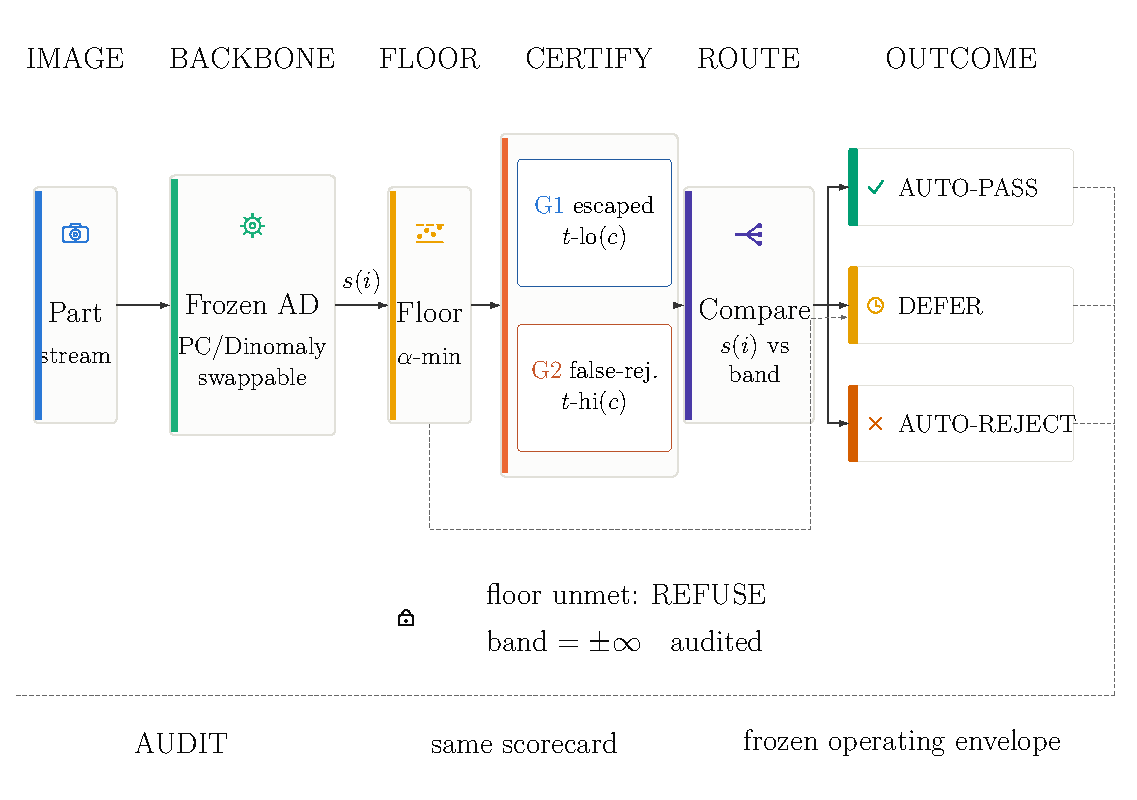
\includegraphics[width=\linewidth]{figures/fig-overview.pdf}
  \caption{Horizontal method overview. A frozen, interchangeable PatchCore or Dinomaly backbone
  scores each image. Per-category calibration first checks the certifiability floor
  $\alpha_{\min}=1/(n_{\text{cal}}+1)$ (Section~\ref{sec:floor}); when met, the parallel G1 and G2
  cards set $t_{\text{lo}}(c)$ and $t_{\text{hi}}(c)$ so that
  $P(s\!\le\!t_{\text{lo}}\mid\text{defective})\le\alpha_{\text{miss}}$ and
  $P(s\!\ge\!t_{\text{hi}}\mid\text{good})\le\alpha_{\text{fr}}$, respectively
  (Section~\ref{sec:gate}). Comparing $s_i$ with this band routes the part to auto-pass, defer, or
  auto-reject. The dashed floor-control branch is distinct from that data path: an unmet floor
  refuses the axis (band $=\pm\infty$), records audited-not-certified, and forces defer rather than
  auto-reject. All three outcomes feed the same audit scorecard and frozen operating envelope; the
  schematic makes no claim that either backbone is superior.}
  \label{fig:overview}
\end{figure}

We state the evidence boundary explicitly. The preregistration was frozen before confirmatory analysis;
MVTec AD is the confirmatory benchmark, while VisA and MPDD are exploratory additions run
under the same protocol. The frozen G2 train-holdout remedy is reported separately, and no
uncomputed result is used in the claims.

\subsection{A calibration/refusal protocol on academic AD benchmarks}
The gate's output is an auditable calibration/refusal protocol: for every product
category it materialises explicit, machine-readable operating parameters --- the two calibrated
thresholds $(\lambda_{\text{pass}}, \lambda_{\text{reject}})$, the certified error budgets
$(\alpha_{\text{miss}}, \alpha_{\text{fr}})$ they enforce, and, where calibration data cannot
support the request, an \emph{audited-not-certified} refusal state --- which downstream
quality-control logic (routing, re-inspection staffing, audit trails) can consume. The
schema is backbone-agnostic: swapping the detector changes the scores, not the form of the
envelope, and the refusal state is an explicit operating signal rather than an implementation
detail. The academic benchmarks used here validate this calibration-and-refusal machinery on
standard AD splits; applying the same schema to production-line data with temporal drift remains
future work (Section~\ref{sec:limitations}).

\section{Related work}
\label{sec:related}

\paragraph{Distribution-free risk control.} The gate is an application of conformal
prediction~\citep{vovk2005algorithmic,lei2018distribution,angelopoulos2023gentle}: given an
exchangeable calibration set, an order statistic of the calibration scores yields a threshold with
a finite-sample coverage guarantee. The specific ingredient we use is the split (inductive)
conformal construction~\citep{papadopoulos2002inductive}, whose single calibration/estimation split
makes it cheap enough to apply per category at deployment time. Set-valued and adaptive variants of
the same idea --- least-ambiguous set-valued classifiers with a bounded error
level~\citep{sadinle2019least} and adaptive-coverage prediction
sets~\citep{romano2020aps} --- show how a one-sided error target maps onto a calibrated threshold,
which is exactly the primitive our two certificates specialise. The broader risk-controlling line
--- risk-controlling prediction sets~\citep{bates2021rcps} and
Learn-then-Test~\citep{angelopoulos2021ltt} --- generalizes this to bounding arbitrary monotone
risks and to multiple-hypothesis calibration. All of these guarantees are conditional on
exchangeability between calibration and deployment data; conformal prediction under covariate
shift~\citep{tibshirani2019covariate} characterises what breaks when that assumption fails, and is
the lens through which we frame threshold-transfer across production periods as future work
(Section~\ref{sec:limitations}). Our escaped-defect and false-reject bounds are the two one-sided
special cases that split conformal already delivers exactly (Section~\ref{sec:gate}); we
deliberately use the simplest sufficient construction rather than the more general
risk-controlling prediction sets / learn-then-test (RCPS/LTT)
machinery, and cite the latter as the family the method belongs to.

\paragraph{Industrial anomaly detection.} MVTec AD~\citep{bergmann2019mvtec} defined the
per-category unsupervised setting we use, and the field it seeded is now broad enough to warrant
dedicated surveys~\citep{liu2024survey}. The dominant families all emit an image- or pixel-level
anomaly score our gate can consume unchanged: memory-bank and feature-distribution methods such as
PatchCore~\citep{roth2022patchcore}, PaDiM~\citep{defard2021padim}, and
SPADE~\citep{cohen2020spade}; student--teacher and knowledge-distillation methods such as uninformed
students~\citep{bergmann2020uninformed} and reverse distillation~\citep{deng2022reverse};
reconstruction and synthetic-defect methods such as DR{\AE}M~\citep{zavrtanik2021draem} and
CutPaste~\citep{li2021cutpaste}; normalizing-flow methods such as
FastFlow~\citep{yu2021fastflow}; and recent simplified or transformer models such as
SimpleNet~\citep{liu2023simplenet} and Dinomaly~\citep{guo2025dinomaly}. Of these, PatchCore and
Dinomaly are the two reproduced backbones here; EfficientAD~\citep{batzner2024efficientad} is a fast
alternative we discuss but do not certify (its only public implementations are community
reimplementations, so it cannot anchor a binding reproduction gate). Dinomaly descends from the
multi-class (one model, many categories) line initiated by UniAD~\citep{you2022unified} --- the
setting its published VisA figure reports and the one we use on VisA
(Section~\ref{sec:setup}). In the applied inspection literature, this
detector line has been carried directly into deployable inspection systems: component-aware anomaly
detection for logical industrial inspection~\citep{liu2023component}, defect-aware transformer
networks for visual surface-defect detection~\citep{shang2023defect}, and autoencoder-based surface
anomaly inspection~\citep{tsai2021autoencoder}, alongside segmentation-based deep-defect
detection~\citep{tabernik2020segmentation} and broader automated-visual-inspection
surveys~\citep{czimmermann2020visual}. That body of work optimises the \emph{detector}; our
contribution is the orthogonal decision layer that sits on top of any such detector's scores and
attaches a certified routing guarantee. MPDD~\citep{jezek2021mpdd} adds a real painted-metal-parts
fabrication benchmark whose non-homogeneous backgrounds and small good pools make it a deliberately
harsher industrial-realism stress test than the two academic staples --- though, like them, still an
academic benchmark rather than production-line data (see Limitations, Section~\ref{sec:limitations}).
We use
anomalib~\citep{akcay2022anomalib} for the PatchCore implementation. Our contribution is orthogonal
to all of these: we consume their scores and add a decision layer, and we improve none of them.

\paragraph{Selective prediction and abstention.} The defer action is a selective-prediction
mechanism~\citep{geifman2017selective,geifman2019selectivenet}, but applied at the decision layer
with a two-sided, per-category certificate rather than a single accuracy-coverage curve or a learned
reject head; the auto-reject certificate (false-reject control) has no analogue in standard
selective classification, which abstains only around the positive decision.

\paragraph{Conformal anomaly detection and abstention.} Conformal methods have been applied to
anomaly detection before, but not to the certified inspection-triage decision we target. Early
work bounded false-alarm rates for sequential and trajectory
anomalies~\citep{laxhammar2011sequential,laxhammar2015inductive}; recent tooling controls the
false-discovery rate over flagged anomalies~\citep{hennhofer2026nonconform}; conformal risk
control~\citep{angelopoulos2022crc} and its graph instantiation
CRC-SGAD~\citep{bai2025crcsgad} bound a monotone risk (e.g.\ false-negative rate/false-positive rate, FNR/FPR) but emit a single flag, not
a three-way route; and dual-threshold conformal abstention for autonomous-system
perception~\citep{kumar2025beyond} adds a reject option on camera/LiDAR (and classification)
tasks, with no industrial-inspection estimand and no evaluation on MVTec AD. Stated plainly,
our delta over that dual-threshold line is not conformal machinery but the inspection
instantiation: the two error axes named and certified as escaped-defect and false-reject
budgets, per-category certifiability floors with first-class refusal, and the audited
deployment protocol around them. The closest defect-detection application~\citep{shen2025conformal} controls a mean error rate for
pixel-level surface-defect segmentation, using recall/false-discovery-rate (FDR)-style losses, whereas this paper
operates on image-level anomaly scores and certifies a three-way triage with abstention plus
explicit per-category sample-size certifiability floors. It therefore differs in substrate,
route, and the operating-state refusal rule; it does not claim pixel-level segmentation
control.
no published method delivers a certified \emph{three-way} triage (auto-pass / auto-reject / defer)
on MVTec AD with \emph{coupled} escaped-defect and false-reject guarantees and explicit
per-category certifiability floors; the preregistered K6 scoop gate, run as a fresh pre-submission
re-scan after the freeze, confirms this --- the closest published
systems~\citep{kumar2025beyond,bai2025crcsgad,shen2025conformal} each differ on a load-bearing axis
(substrate, estimand coupling, or the defer option), and two adjacent 2026 works ---
Yu and Liu's selective-risk certificate on generic vision~\citep{yu2026selective} and
Yuan et al.'s conformal cyber-physical-systems detector on sensor
time-series~\citep{yuan2026conformal} --- target neither the image-inspection estimand nor the
three-way route. That
is the seam this paper occupies. Section~\ref{sec:crcbaseline} instantiates the single-threshold
CRC construction~\citep{angelopoulos2022crc} as a quantitative baseline on our own canonical score
dumps under the identical protocol, isolating what the three-way route and its coupled
false-reject certificate add over the nearest single-flag alternative. Our validation is on academic benchmarks;
deployment on production lines with temporal drift and non-stationary defect arrival is future work (Section~\ref{sec:limitations}).

\section{Methods}
\label{sec:methods}

Table~\ref{tab:glossary} collects the short-codes reused throughout
Sections~\ref{sec:methods}--\ref{sec:limitations}, as a single reference point instead of a
re-derivation on each reuse.

\begin{table}[htbp]
  \centering
  \footnotesize
  \caption{Notation and short-code glossary. Every code below recurs at least twice in
  Sections~\ref{sec:methods}--\ref{sec:limitations}; consult this table rather than re-deriving a
  code's meaning from context on each reuse.}
  \label{tab:glossary}
  {\renewcommand{\arraystretch}{0.88}
  \begin{tabular}{@{}l >{\raggedright\arraybackslash}p{0.80\linewidth}@{}}
    \toprule
    Code & Meaning \\
    \midrule
    G1 & Certified escaped-defect bound (Section~\ref{sec:gate}) \\
    G2 & Certified false-reject bound (Section~\ref{sec:gate}) \\
    K1--K7 & Kill-gates: coverage sanity, vacuity, backbone floor ($\ge 0.90$ AUROC), audit
      headroom, calibration floor, prior-work re-scan, compute guard (in order) \\
    V1 tier-1 & Validity audit: certificate-validity statistic \\
    V1 tier-2 & Validity audit: stringent Clopper--Pearson estimator-variance readout \\
    A1--A3 & Amendments: (A1) tier-2 power floor graded per repeat, not pooled; (A2) near-target
      tier-2 estimator variance is expected, not failure; (A3) false-reject axis graded only over
      G2-certified cells \\
    B1/B2/B3 & Threshold practices: (B1) single global fixed threshold; (B2) per-category tuned
      threshold; (B3) train-good quantile threshold \\
    C2 & Confirmatory excess-AURC audit (pooled Holm family, Section~\ref{sec:c2}) \\
    CRC & Conformal Risk Control, the single-threshold conformal baseline \\
    \bottomrule
  \end{tabular}}
\end{table}
\FloatBarrier

\subsection{The three-way gate and its two certificates}
\label{sec:gate}

Each image $i$ in category $c$ has an anomaly score $s_i$ with the convention \emph{higher
$=$ more anomalous}. The gate is a pair of per-category thresholds $(t_{\text{lo}}(c),
t_{\text{hi}}(c))$ with $t_{\text{lo}} \le t_{\text{hi}}$: images with $s_i \le t_{\text{lo}}(c)$
auto-pass, images with $s_i \ge t_{\text{hi}}(c)$ auto-reject, and the rest defer. (If a refusal or
crossed thresholds leave the auto-reject band empty, the overlap simply defers, and both guarantees
still hold.)

Equivalently, Equation~\eqref{eq:threewaydecision} reports the decision for image $i$:
\begin{equation}
D(s_i;c)=
\begin{cases}
\text{pass}, & s_i \le t_{\text{lo}}(c),\\
\text{reject}, & s_i \ge t_{\text{hi}}(c),\\
\text{defer}, & t_{\text{lo}}(c) < s_i < t_{\text{hi}}(c).
\end{cases}
\label{eq:threewaydecision}
\end{equation}

\paragraph{G2 --- certified false-reject, directly.} $t_{\text{hi}}(c)$ is the split-conformal
upper quantile of the \emph{good} calibration scores at level $\alpha_{\text{fr}}$
~\citep{papadopoulos2002inductive,vovk2005algorithmic}: with
$n_{\text{cal}}^{\text{good}}$ good calibration scores, Equation~\eqref{eq:g2quantile} sets it to
the order statistic at rank
$\lceil (n+1)(1-\alpha_{\text{fr}}) \rceil$, guaranteeing $P(s \ge t_{\text{hi}} \mid \text{good})
\le \alpha_{\text{fr}}$ under exchangeability as in Equation~\eqref{eq:g2guarantee}. This is exactly
the split-conformal upper-quantile construction applied to the good scores.
\begin{equation}
t_{\text{hi}}(c)=S^{\text{good}}_{(k_{\text{hi}})},\qquad
k_{\text{hi}}=\left\lceil \bigl(n_{\text{cal}}^{\text{good}}+1\bigr)
\bigl(1-\alpha_{\text{fr}}\bigr)\right\rceil ,
\label{eq:g2quantile}
\end{equation}
\begin{equation}
\Pr\!\left\{s \ge t_{\text{hi}}(c)\mid \text{good},\,c\right\}
\le \alpha_{\text{fr}} .
\label{eq:g2guarantee}
\end{equation}
% implemented by the split-conformal routine relmetrics.conformal.SplitConformal

\paragraph{G1 --- certified escaped-defect, by negation.} Bounding
$P(s \le t_{\text{lo}} \mid \text{defective})$ is the mirror image: apply the same split-conformal
construction~\citep{papadopoulos2002inductive} to the \emph{negated} defective calibration scores $Y=-X$ at level
$\alpha_{\text{miss}}$, then map the resulting upper quantile back through the negation. The gate
module proves the order-statistic identity in Equation~\eqref{eq:g1mirror}, and it is checked against the design's
$\lfloor \alpha(n+1)\rfloor$ formula in the accompanying unit tests. No new
estimator is introduced; both certificates are the same conformal quantile.
\begin{equation}
\begin{aligned}
&t_{\text{lo}}(c)=-Y_{(k_{\text{lo}})},\qquad
Y=-X,\qquad
k_{\text{lo}}=\left\lceil \bigl(n_{\text{cal}}^{\text{def}}+1\bigr)
\bigl(1-\alpha_{\text{miss}}\bigr)\right\rceil ,\\[2pt]
&\Pr\!\left\{s \le t_{\text{lo}}(c)\mid \text{defective},\,c\right\}
\le \alpha_{\text{miss}} .
\end{aligned}
\label{eq:g1mirror}
\end{equation}
% source: README.md "The gate: zero new math"; proof in inspect_gate/gate.py module docstring; checked in tests/test_gate.py

\paragraph{Mondrian per-category stratification.} Calibration is stratified by category (a Mondrian
conformal construction~\citep{vovk2005algorithmic}): each category gets its own $(t_{\text{lo}}, t_{\text{hi}})$, so the
guarantee is conditional on category, not marginal. An optional finer per-defect-type
stratification is exploratory only (Section~\ref{sec:limitations}).

\paragraph{Where the labeled defectives come from.} G1 calibrates on labeled \emph{defective}
images per category ($n_{\text{cal}}^{\text{def}}$ in Table~\ref{tab:floors}) --- a requirement
unsupervised anomaly detection is deployed specifically to avoid needing at detector-training
time, since labeled defects are scarce, especially early in a line's life. This is a real cost
relative to the unsupervised premise: the certificate is only as good as the labeled defective
pool behind it, and unlike the detector itself that pool cannot be assembled from good parts
alone. In deployment it is not a fixed benchmark quantity but accrues over time, from rework,
scrap, and quality-escape logs as the line runs. The $\alpha_{\min}=1/(n_{\text{cal}}^{\text{def}}+1)$
floor and the refusal rule below are what make this honest rather than aspirational: a category
with a thin defect history is refused and reported audited-not-certified rather than issued a
certificate its data cannot support, and MPDD's connector category already demonstrates the
mechanism in practice ($n_{\text{cal}}^{\text{def}}=7 < 9$ at $\alpha_{\text{miss}}=0.10$, refused
at the frozen rate; Section~\ref{sec:floors}).

\subsection{Certifiability floors and refusal}
\label{sec:floor}

Split conformal cannot certify an arbitrarily small rate from a finite calibration pool: the
smallest achievable level is $\alpha_{\min} = 1/(n_{\text{cal}}+1)$. A category is certifiable for a
guarantee iff $\alpha_{\min} \le \alpha$ as in Equation~\eqref{eq:certfloor}; otherwise the gate
\emph{refuses}, setting the corresponding threshold to $\pm\infty$ (the band is empty, all such
images defer) and marking the category audited-not-certified for that axis. Refusal is emitted,
never rounded away:
\begin{equation}
\alpha_{\min}(n_{\text{cal}})=\frac{1}{n_{\text{cal}}+1},
\qquad
\text{certifiable at level }\alpha
\iff
\alpha_{\min}(n_{\text{cal}})\le \alpha .
\label{eq:certfloor}
\end{equation}
% source: PREREG-DRAFT-2026-07-10.md §2--§3 (alpha_min = 1/(n_cal+1)); README.md "Honest-uncertainty rules"
This is the honesty rule that makes the floor table (Section~\ref{sec:floors}) a result rather
than a limitation.

The gate's mechanism is made concrete on one repeat of the frozen protocol in Figure~\ref{fig:scoreanatomy}.
\begin{figure}[htbp]
\centering
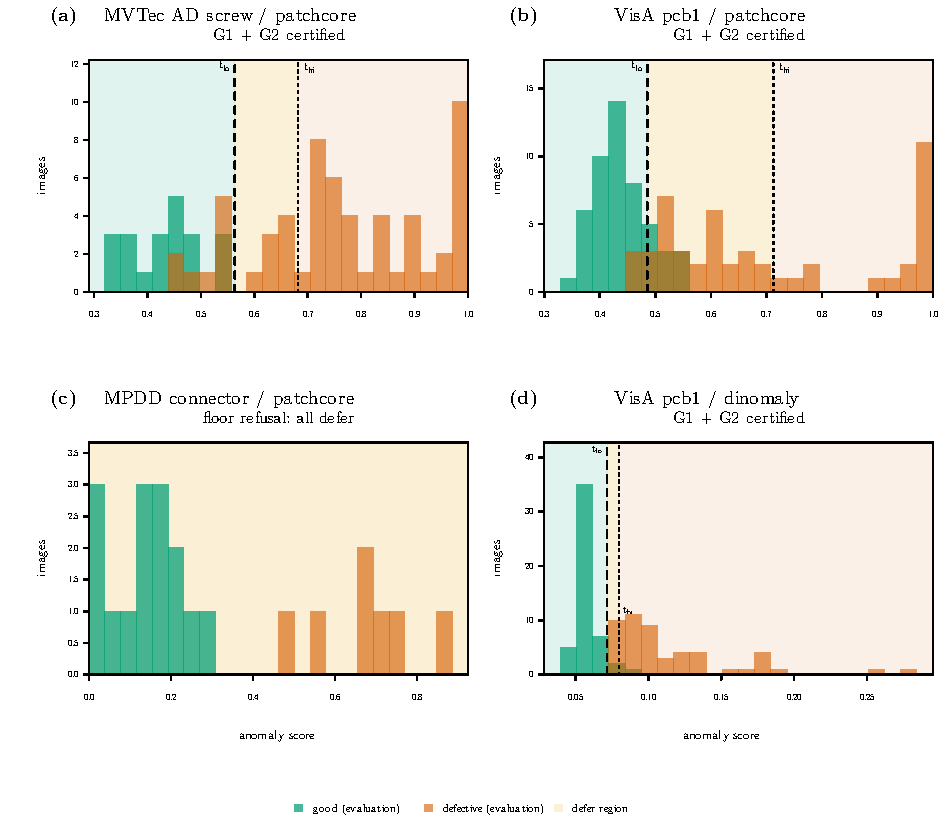
\includegraphics[width=0.97\linewidth]{figures/fig-scoreanatomy.pdf}
\caption{The gate's mechanism on real scores (seed $0$, repeat $0$; evaluation-half
histograms, thresholds calibrated on the calibration half). \textbf{a:}~MVTec AD screw
(PatchCore): both certificates, defer band absorbs the overlap region. \textbf{b:}~VisA
pcb1 (PatchCore): both certified with a wider band. \textbf{c:}~MPDD connector
(PatchCore): separation looks clean to the eye yet the gate refuses --- pools too small
for the $1/(n_{\text{cal}}+1)$ floors, both thresholds at $\pm\infty$. \textbf{d:}~VisA
pcb1 under \emph{Dinomaly} (contrast with b): same category, different scorer; both G1
and G2 certify with a narrow band ($t_{\text{lo}}=0.072$, $t_{\text{hi}}=0.080$), showing
that a different detector with cleaner score separation can close the defer band
substantially.}
\label{fig:scoreanatomy}
\end{figure}

Figure~\ref{fig:scoreanatomy} makes the mechanism concrete on one repeat of the frozen protocol:
where the two score masses are well separated the band is narrow and both certificates issue
(panel a); where they overlap the band widens to cover the overlap and deferral rises (panel b);
and where calibration pools are too thin the gate refuses outright (panel c) --- the refusal
reads the pool sizes, not the apparent separability, which is precisely why a threshold picked
by eye on panel c would be an uncertified decision the gate declines to automate.

\subsection{Validity audit (V1) and kill-gates (K1--K7)}
\label{sec:v1}

We fix $\alpha_{\text{miss}}=0.10$ and $\alpha_{\text{fr}}=0.05$ throughout, with a $+3$pp
estimator tolerance (thresholds $0.13$ / $0.08$) and $95\%$ one-sided Clopper--Pearson
intervals~\citep{clopper1934use}.
% source: PREREG-DRAFT-2026-07-10.md §2 (frozen targets table)
The \emph{validity audit} V1 has two tiers. Tier-1 checks that the realized mean escaped-defect and
false-reject rates in Equation~\eqref{eq:v1rates} lie within target$+3$pp over repeated
calibration/evaluation splits; this is the certificate-validity statistic. Tier-2 forms the
Clopper--Pearson upper bound in Equation~\eqref{eq:cpupper} and is graded, per the frozen
amendments, as a stringent estimator-variance readout (Section~\ref{sec:tier2verdict}),
because on MVTec AD its power floor is not met per repeat and its tolerance is near-unpassable by
construction for a correctly-calibrated gate. The manuscript-level V1 family contains
$33\times2\times5=330$ benchmark--category--backbone--seed cells (MVTec AD $15$, VisA $12$, MPDD
$6$ categories; two backbones; five seeds). We therefore keep the confirmatory inferential claims
separate from this diagnostic grid: V1 reports deterministic pass/fail counts, finite-sample power
exclusions, and one-sided Clopper--Pearson intervals, while the only hypothesis-test family used to
claim practice skill is the C2 Holm-adjusted excess-AURC audit (Section~\ref{sec:c2}). Post-freeze
VisA/MPDD V1 cells are labelled exploratory and are not pooled into the frozen MVTec confirmatory
family.
\begin{equation}
\begin{aligned}
\widehat r_{\text{miss}}
&=\frac{1}{|\mathcal E_{\text{def}}|}
\sum_{i\in\mathcal E_{\text{def}}}\mathbf{1}\{D(s_i;c_i)=\text{pass}\},\\[2pt]
\widehat r_{\text{fr}}
&=\frac{1}{|\mathcal E_{\text{good}}|}
\sum_{i\in\mathcal E_{\text{good}}}\mathbf{1}\{D(s_i;c_i)=\text{reject}\}.
\end{aligned}
\label{eq:v1rates}
\end{equation}
\begin{equation}
U_{\text{CP}}(k,m;\gamma)=
\begin{cases}
\operatorname{Beta}^{-1}_{1-\gamma}(k+1,m-k), & k<m,\\
1, & k=m,
\end{cases}
\qquad \gamma=0.05 .
\label{eq:cpupper}
\end{equation}

A battery of preregistered kill-gates guards the construction: K1 (coverage sanity --- halt if
tier-1 fails in $\ge 5$ of the $15\!\times\!B$ cells), K2 (vacuity --- kill if median deferral
$>0.80$ in $\ge 8/15$ categories on all backbones), K3 (backbone floor --- mean image-AUROC
$\ge 0.90$), K4 (audit headroom), K5 (calibration floor --- fires only if $\alpha_{\min}>0.10$ in
$\ge 3$ categories), K6 (a citation re-scan for a prior certified triage), and K7 (a compute guard).
% source: PREREG-DRAFT-2026-07-10.md §5, §7.1 (falsification conditions)

\subsection{Excess-AURC audit}
\label{sec:audit}

Beyond validity, we ask whether standard thresholding practice earns deferral skill at all.
For each practice --- B1 (global fixed threshold), B2 (per-category tuned), B3 (train-good quantile)
--- we compare its area-under-the-risk-coverage-curve against the closed-form random-deferral null
(evaluated in closed form, never Monte-Carlo'd), with the statistic in
Equation~\eqref{eq:aurcstat}, using a matched-abstention,
% closed-form random-deferral AURC null: relmetrics.aurc.random_aurc
category-stratified permutation $p$-value ($2000$ permutations), a category-blocked bootstrap CI,
and a roster-derived Holm~\citep{holm1979simple} correction. The verdict is symmetric: if no
practice beats random the paper reports a debunking finding; if all do it reports a constructive one.
\begin{equation}
\begin{aligned}
\widehat C_{\pi}(\tau)
&=\frac{1}{|\mathcal E|}\sum_{i\in\mathcal E} A_{\pi,\tau}(i),\\
\widehat R_{\pi}(\tau)
&=\frac{\sum_{i\in\mathcal E} L_i A_{\pi,\tau}(i)}
{\sum_{i\in\mathcal E} A_{\pi,\tau}(i)},\\
\widehat{\operatorname{AURC}}(\pi)
&=\int_0^1 \widehat R_{\pi}(u)\,du,\\
\widehat\Delta_{\text{AURC}}(\pi)
&=\widehat{\operatorname{AURC}}(\pi)
-\widehat{\operatorname{AURC}}(\text{random deferral}).
\end{aligned}
\label{eq:aurcstat}
\end{equation}
% source: PREREG-DRAFT-2026-07-10.md §7 step 7; README.md audit.py

\section{Experimental setup}
\label{sec:setup}

\paragraph{Data.} Three public benchmarks. MVTec AD~\citep{bergmann2019mvtec}: $15$
object/texture categories, $3{,}629$ train-good images, and a test set of $467$ good $+$
$1{,}258$ defective $=$ $1{,}725$ images across $73$ defect types. VisA~\citep{zou2022spot},
under the official one-class \texttt{spot-diff} split: $12$ categories, $8{,}659$ train-good
images, and a test set of $962$ good $+$ $1{,}200$ anomalous $=$ $2{,}162$ images (VisA's
public ground truth carries a single ``bad'' stratum per category, so the defect-type Mondrian
axis is unavailable there). MPDD~\citep{jezek2021mpdd} (post-freeze exploratory; see below):
$6$ real painted-metal-part categories, $888$ train-good images, and a test set of $176$ good
$+$ $282$ defective $=$ $458$ images from a public release mirrored for staging. Splits follow
each benchmark's official protocol, or a frozen per-category test manifest where none ships;
score records are joined to those splits with refusal on any missing or extra image.
% official 1-class split file: 1cls.csv; box builder: orchestration/visa_prep.py;
% score-dump adapter: visa_results_2026-07-12/scripts/visa_adapter.py
% MPDD source + sha256: DATA_MANIFEST.md (meksamiao/mpdd, archive_sha256 in mpdd_split_manifest.json);
% MPDD adapter: mpdd_results_2026-07-13/scripts/mpdd_adapter.py -> ADAPTER-REPORT.json
% source: PREREG-DRAFT-2026-07-10.md §2 (data provenance); §7 step 1;
% visa_results_2026-07-12/ADAPTER-REPORT.json (official_test_counts)

Figure~\ref{fig:samples} illustrates the three-way decisions on real parts across the route and ground-truth classes.
\begin{figure}[htbp]
\centering
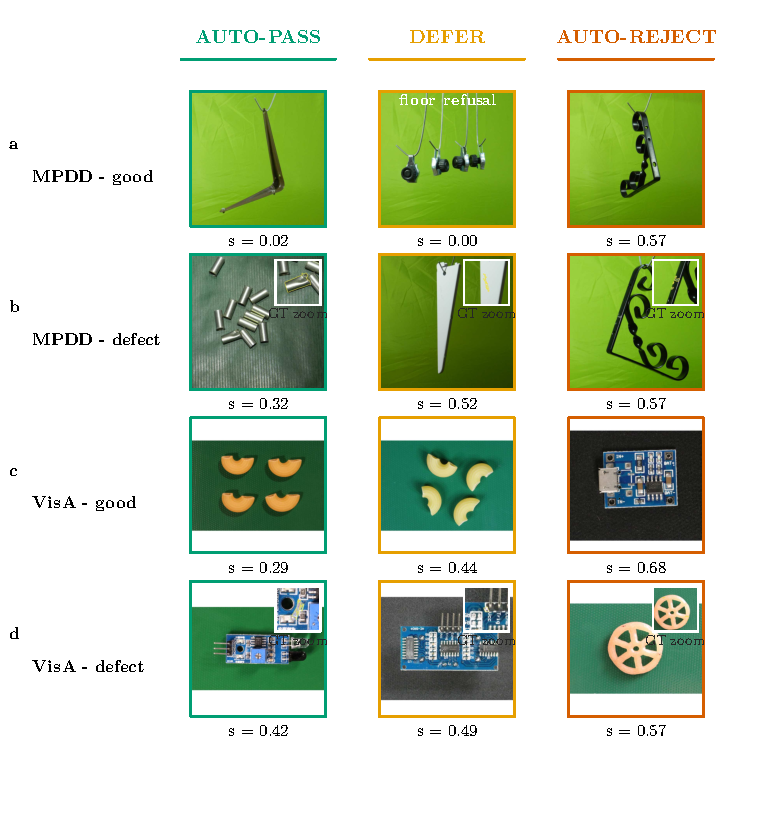
\includegraphics[width=0.92\linewidth]{figures/fig-samples.pdf}
\caption{Three-way decisions on real parts (PatchCore, seed 0, repeat-0 split;
illustrative, not a new experiment). Columns show auto-pass, defer, and
auto-reject; rows show MPDD good, MPDD defective, VisA good, and VisA
defective examples. Border color encodes the route and each tile gives its
anomaly score. Insets and yellow contours use dataset ground truth to locate
defects and are not model localization. MPDD uses the train-holdout rescue arm
(Section~\ref{sec:mpddholdout}); VisA uses the primary protocol. The connector defer tile
is marked \emph{floor refusal}: connector's escaped-defect side cannot certify at
$\alpha_{\text{miss}}=0.10$ ($\alpha_{\min}=0.125$), so $t_{\text{lo}}=-\infty$ and every image
defers --- a different decision class from a within-band defer, which the tile now names
explicitly. Together the
examples expose all six ground-truth/route classes, including false rejection
and escaped-defect cases.}
\label{fig:samples}
\end{figure}

\paragraph{Backbones (Branch A, $B=2$).} PatchCore~\citep{roth2022patchcore} via
anomalib~\citep{akcay2022anomalib} (a Wide ResNet-50-2 backbone, features from the second and
third stages, coreset ratio $0.10$)\footnote{Target $0.991$ is PatchCore's published
$25\%$-coreset mean; we score the $10\%$-coreset point (PREREG~D3).
See Table~\ref{tab:repro}.} and Dinomaly~\citep{guo2025dinomaly} (canonical score dump,
its own eval script; on VisA, the reference repo's multi-class setting --- one model per seed for
all $12$ categories --- which is the setting its published VisA figure reports). Both were
confirmed present and reproduction-passing before any calibration, so the preregistered
two-backbone branch (Branch A) is active; the same two backbones and configurations are used
unchanged on VisA.
% source: PREREG-DRAFT-2026-07-10.md §1--§2; ANALYSIS-MEMO.md §1
\paragraph{Protocol.} Primary protocol: test-side good calibration, no
train-holdout. For each (backbone, category, seed) we draw $R=20$ stratified $50/50$
% primary-protocol CLI flag: --good-cal test
calibration/evaluation splits (split-seed $=$ repeat index), with $5$ backbone seeds ($0$--$4$).
% source: PREREG-DRAFT-2026-07-10.md §2 (split protocol)

\section{Results}
\label{sec:results}

All numbers in this section are recomputed from the frozen local score dumps by the archived
analysis pipeline --- a MVTec AD analysis stage, a stage-identical VisA analysis stage, a
stage-identical MPDD analysis stage (with its own train-holdout rescue stage), and the
G2-promotion stage, each emitting a frozen result summary; none is trusted from a training log or
the literature.
% MVTec: analysis_2026-07-10/scripts/run_analysis.py -> analysis_2026-07-10/SUMMARY.json;
% VisA: visa_results_2026-07-12/scripts/run_visa_analysis.py -> visa_results_2026-07-12/SUMMARY.json;
% MPDD: mpdd_results_2026-07-13/scripts/run_mpdd_analysis.py -> SUMMARY.json;
%       mpdd_results_2026-07-13/scripts/run_mpdd_holdout_analysis.py -> HOLDOUT-RESULTS.json;
% G2 promotion: g2_promotion_2026-07-12/run_g2_promotion.py

\subsection{Reproduction gate}
\label{sec:repro}

On all three benchmarks the gate recomputes image-AUROC (Mann--Whitney rank-sum identity) directly
from the local scores and compares it against a named published target (Table~\ref{tab:repro}).
On MVTec AD both backbones pass in all $5$ seeds, and K3 (mean AUROC $\ge 0.90$) holds with wide
margin. On VisA, Dinomaly passes in all $5$ seeds against its own published VisA figure
($0.987$, multi-class setting), and our recomputation again reproduces its reported per-seed
mean image-AUROC seed for seed (max per-category deviation $3.3\times 10^{-5}$ over
% reproduced value: the training-log "Mean: I-Auroc" line
all $60$ seed$\times$category cells). PatchCore has no repo-confirmed published VisA figure, so
per the tool's no-guessed-target rule its VisA row is \emph{descriptive} (no pass/fail is
graded); its recomputed mean of $0.903$--$0.908$ still clears the K3 floor, though with thin
margin (seed $3$: $0.9033$, i.e.\ $0.33$pp above the $0.90$ floor), and the drop from $0.982$
(MVTec) is exactly the lower-ceiling substrate the audit needs (Section~\ref{sec:auditres}). On
MPDD, Dinomaly passes in all $5$ seeds against its published MPDD multi-class figure ($0.972$;
recomputed mean $0.9712$--$0.9738$, grand mean $0.9722 \pm 0.0010$), our recomputation matching
the box's per-category training-log AUROC to $\le 4.9\times10^{-5}$; PatchCore-on-MPDD has no
repo-confirmed published figure, so per the same no-guessed-target rule its row is
descriptive (recomputed mean $0.948$--$0.957$).
% source: analysis_2026-07-10/SUMMARY.json["reproduction"]; ANALYSIS-MEMO.md §1;
% visa_results_2026-07-12/SUMMARY.json["reproduction"]; ADAPTER-REPORT.json (xcheck)
% MPDD: mpdd_results_2026-07-13/SUMMARY.json["reproduction"] (+seed_stability_summary);
%   ADAPTER-REPORT.json (auroc_xcheck max_abs_diff 4.9e-5; per-seed maxima 4.3/4.4/3.2/4.9/4.9e-5)

\begin{table}[htbp]
  \centering
  \caption{Reproduction gate, $5$ seeds per backbone per benchmark. Mean image-AUROC range is
  over seeds; the weakest category is named. ``n/a'': no repo-confirmed published
  PatchCore-on-VisA/MPDD figure exists, so that row is descriptive by design (no pass/fail graded).
  Recomputed from the frozen MVTec AD, VisA, and MPDD analysis summaries.}
  % source: analysis_2026-07-10, visa_results_2026-07-12, mpdd_results_2026-07-13 SUMMARY.json["reproduction"]
  \label{tab:repro}
  \small
  \resizebox{\linewidth}{!}{%
  \begin{tabular}{l l c >{\raggedright\arraybackslash}p{0.15\textwidth} >{\raggedright\arraybackslash}p{0.18\textwidth} c}
    \toprule
    Benchmark & Backbone & Target ($\pm 0.02$) & Mean I-AUROC (seed range) & Weakest category & Gate \\
    \midrule
    MVTec AD & PatchCore & 0.991 & 0.9817--0.9826 & toothbrush 0.911--0.917 & PASS 5/5 \\
    MVTec AD & Dinomaly  & 0.996 & 0.9957--0.9965 & capsule 0.976--0.982    & PASS 5/5 \\
    VisA     & PatchCore & n/a   & 0.9033--0.9083 & macaroni2 0.656--0.665  & descriptive \\
    VisA     & Dinomaly  & 0.987 & 0.9866--0.9876 & macaroni2 0.956--0.966  & PASS 5/5 \\
    MPDD     & PatchCore & n/a   & 0.9481--0.9568 & bracket black 0.872--0.888 & descriptive \\
    MPDD     & Dinomaly  & 0.972 & 0.9712--0.9738 & bracket black 0.929--0.940 & PASS 5/5 \\
    \bottomrule
  \end{tabular}%
  }
\end{table}
\FloatBarrier

\subsection{Cross-seed stability}
\label{sec:seed}

PatchCore's five seeds are genuinely distinct: all $60$ seed-0-vs-seed-$N$ score-table comparisons
($15$ categories $\times$ $4$ seeds) are $0/60$ bit-identical, with $\max|\Delta\text{score}|$
ranging $0.026$--$0.153$ (mean $0.074$) --- a real but modest variance source, so PatchCore is
reported as a $5$-effective-seed backbone, not collapsed to one. Dinomaly is low-variance: mean
image-AUROC across seeds $0.9960 \pm 0.00029$, with the widest per-category spread only $0.0060$
(capsule). The same picture holds on VisA: PatchCore is $0/48$ bit-identical
($\max|\Delta\text{score}|$ $0.044$--$0.256$), and Dinomaly's mean image-AUROC across seeds is
$0.9870 \pm 0.0004$ with the widest per-category spread $0.0104$ (macaroni2). On MPDD the pattern
repeats once more: PatchCore is $0/24$ bit-identical across the seed-0-vs-seed-$N$ comparisons,
and Dinomaly's mean image-AUROC across seeds is $0.9722 \pm 0.0010$.
% source: analysis_2026-07-10/SUMMARY.json["seed_stability_summary"]; ANALYSIS-MEMO.md §2;
% visa_results_2026-07-12/seed_stability/seed_stability.json;
% mpdd_results_2026-07-13/SUMMARY.json["seed_stability_summary"]

\subsection{Certifiability floors and the G1/G2 split}
\label{sec:floors}

Table~\ref{tab:floors} is the paper's honesty figure. The per-category calibration counts computed
from the full local test arrays match the preregistered arithmetic-only floor table exactly
($0/15$ mismatches for both backbones, identical across all $5$ seeds). At the frozen rates,
escaped-defect (G1) is certifiable in all $15$ categories; false-reject (G2) is certifiable
in exactly $4$ --- cable, hazelnut, screw, transistor --- the categories with
$n_{\text{cal}}^{\text{good}} \ge 19$. The other $11$ categories are refused for G2 and reported
audited-not-certified. We are careful about what this exact match does and does not show: the
per-category counts are a \emph{deterministic} function of the fixed MVTec test split
(round-half-to-even of $n/2$), so the $0/15$ agreement with the preregistered table is a
pipeline-correctness check --- it confirms the data staging re-derives the frozen counts with no
off-by-one or CSV-read error --- not an empirical result about the gate. The genuinely empirical
result is the V1 tier-1 validity audit below (Section~\ref{sec:v1res}), measured from real
calibrate/route/evaluate runs, which could have failed had the calibration or routing pipeline been
broken.
% source: PREREG-DRAFT-2026-07-10.md §3 (floor table); SUMMARY.json["n_cal_count_mismatches_across_seeds"]=0; ANALYSIS-MEMO.md §3

% Table tab:floors appears in the appendix.
\FloatBarrier

\paragraph{VisA: the same arithmetic, a friendlier split.} On VisA the identical floor
computation lands on the opposite side of the ledger: every category's test split carries
$100$ anomalous and $50$--$101$ good images, so after the $50/50$ calibration split
$n_{\text{cal}}^{\text{def}} = 50$ everywhere ($\alpha_{\min}^{\text{G1}} = 0.0196$) and
$n_{\text{cal}}^{\text{good}} \in \{25, 30, 50\}$ ($\alpha_{\min}^{\text{G2}} =
0.0196$--$0.0385$), all below $\alpha_{\text{fr}} = 0.05$. G1 and G2 both certify in
$12/12$ categories under the primary protocol alone --- no train-holdout remedy is needed on
VisA --- and the floors are again identical across both backbones and all five seeds ($0$
mismatches). This is the refusal mechanism working in both directions: it refuses $11/15$
categories on MVTec AD because the data cannot support the rate, and certifies $12/12$ on VisA
because it can.
% source: visa_results_2026-07-12/gate_calibration/v1_*_seed*.json ("certifiability_floors");
% SUMMARY.json["n_cal_count_mismatches_across_seeds"]=0

\paragraph{MPDD: the stingy extreme of pool-size-driven refusal.} MPDD's per-category
test-good pools are uniformly small ($26$--$32$ images $\to n_{\text{cal}}^{\text{good}}$
$13$--$16$, every one below the $19$ the false-reject floor needs at $\alpha_{\text{fr}}=0.05$),
so G2 is certifiable in $0/6$ categories under the primary protocol, on both backbones,
identical across all five seeds ($0$ mismatches). G1 (escaped-defect) stays healthy at $5/6$ ---
only connector fails, its $14$ test-defective yielding $n_{\text{cal}}^{\text{def}}=7<9$.
This places MPDD at the stingy end of three points consistent with pool-size-driven refusal, ordered by good-pool size:
MPDD $0/6 \to$ MVTec AD $4/15 \to$ VisA $12/12$ (all three computed apples-to-apples by
the identical floor code path). MPDD is thus not an intermediate point but the cleanest
demonstration of the paper's thesis --- the certifiable count is a property of how much
exchangeable good data the protocol can spend, and the gate refuses precisely when the data
cannot pay for a $5\%$-false-reject certificate.
% source: mpdd_results_2026-07-13/SUMMARY.json["g2_certifiable_count"]={patchcore:0,dinomaly:0},
%   ["n_cal_count_mismatches_across_seeds"]=0; gate_calibration/v1_*_seed0.json (G1 5/6, connector);
%   FLOOR-PREDICTION.md (trend MPDD 0/6 -> MVTec 4/15 -> VisA 12/12)
Figure~\ref{fig:categorymap} makes this certify-or-refuse pattern visible at the category level
across all three benchmarks: VisA certifies both axes in every category, MVTec AD's false-reject
row is hatched (refused) everywhere except the four categories in Table~\ref{tab:floors}, and
MPDD's false-reject row is hatched throughout --- the visual complement of the same table.

\begin{figure}[htbp]
  \centering
  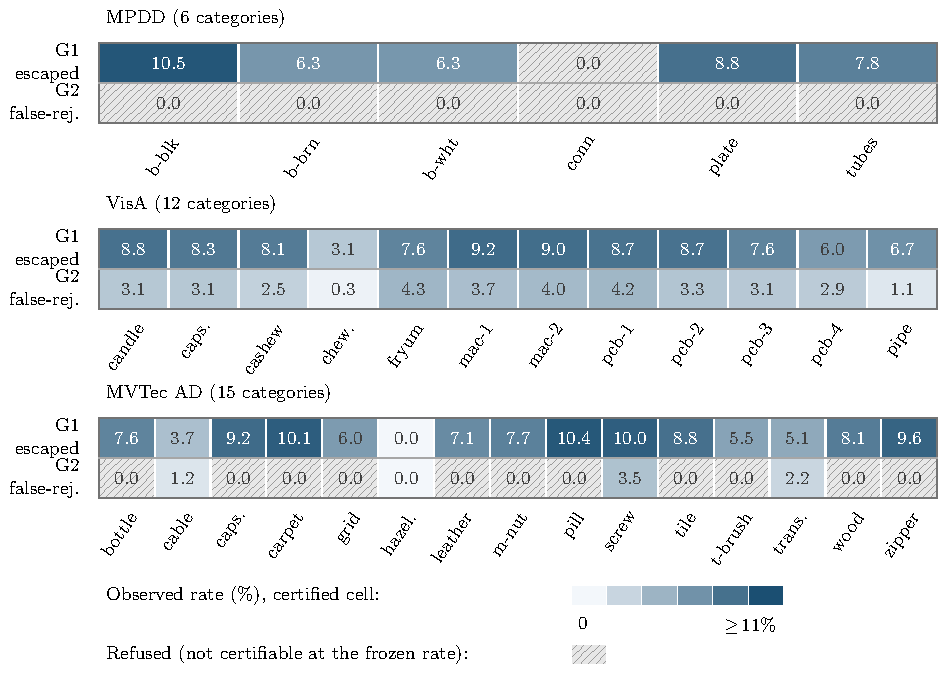
\includegraphics[width=\linewidth]{figures/fig-categorymap.pdf}
  \caption{Per-category certification map for escaped-defect (G1) and false-reject (G2) at the
  frozen rates ($\alpha_{\text{miss}}=0.10$, $\alpha_{\text{fr}}=0.05$), pooled over both backbones
  and five seeds, for MPDD, VisA, and MVTec AD. Colored cells are certified, shaded by the observed
  rate; hatched gray cells are refused as not certifiable at the frozen rate under the primary
  protocol (all of MPDD's G2 row, MPDD's connector on G1, and the $11/15$ MVTec AD categories
  below the false-reject floor in Table~\ref{tab:floors}). A colored $0.0$ is a certified cell
  with zero observed errors; a hatched $0.0$ reports the observed rate but withholds the
  certificate because the calibration floor is unmet. MPDD codes are b-blk/bracket black,
  b-brn/bracket brown, b-wht/bracket white, conn/connector, and plate/metal plate. VisA
  abbreviations are caps./capsules, chew./chewing gum, mac-1/macaroni1, mac-2/macaroni2,
  pcb-1--pcb-4, and pipe/pipe fryum. MVTec AD abbreviations are caps./capsule,
  hazel./hazelnut, m-nut/metal nut, t-brush/toothbrush, and trans./transistor; remaining
  category labels are written in full.}
  \label{fig:categorymap}
\end{figure}

\subsection{The operating-point frontier (post-freeze exploratory)}
\label{sec:frontier}

The post-freeze operating-point sweep is shown in Figure~\ref{fig:alphafrontier}.
\begin{figure}[htbp]
\centering
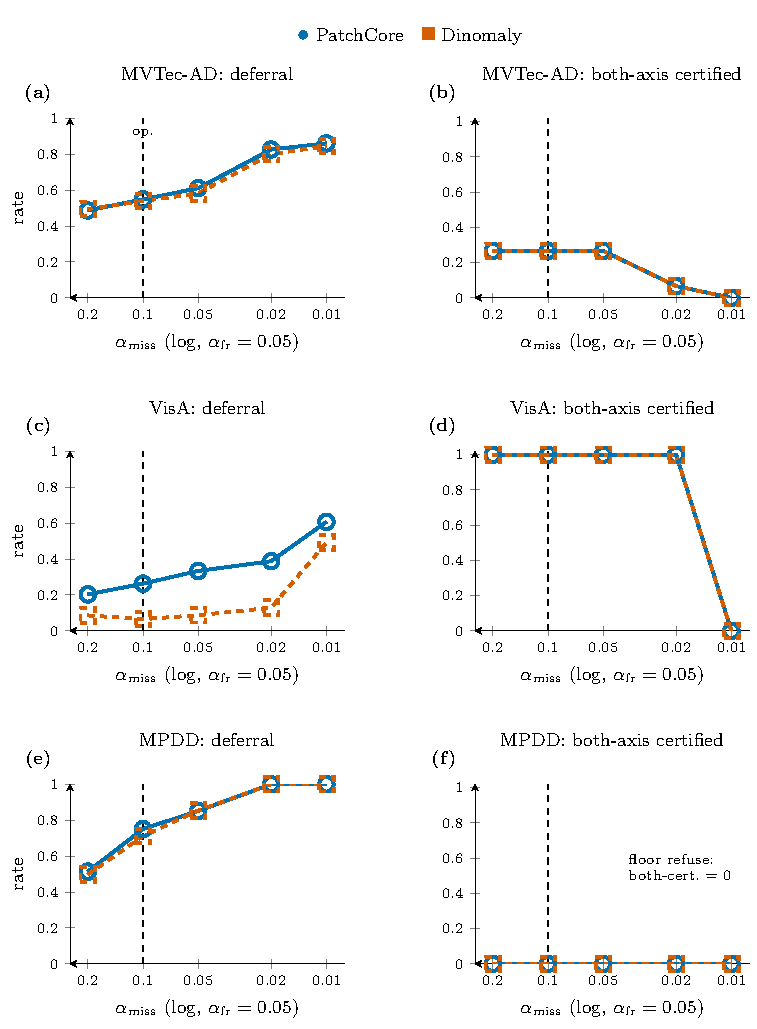
\includegraphics[width=0.92\linewidth]{figures/fig-alphafrontier.pdf}
\caption{The operating-point frontier on the frozen code path (post-freeze exploratory
sweep; the construction reproduces every frozen artifact exactly at the paper's
operating point). Rows are MVTec AD (a,b), VisA (c,d), and MPDD (e,f). Left panels
show mean deferral versus the escaped-defect target $\alpha_{\text{miss}}$ at
$\alpha_{\text{fr}}=0.05$; right panels show the fraction of categories certified on
both axes. Solid circles denote PatchCore and dashed squares Dinomaly; shaded bands
span seed minima to maxima. The vertical dashed line marks the paper's operating point.
The flat zero in panel (f) for MPDD at $\alpha_{\text{miss}}\in\{0.02,0.01\}$ is a
measured refusal: the floor ($\alpha_{\min}=1/(n_{\text{cal}}^{\text{frac}}+1)$) refuses
all six MPDD categories, so both-certified is identically zero on every repeat and
deferral saturates at $1.0$ (no silent decisions).}
\label{fig:alphafrontier}
\end{figure}

The headline rates above all sit at one operating point
($\alpha_{\text{miss}}=0.10$, $\alpha_{\text{fr}}=0.05$). Because a plant will ask what a
tighter escape budget costs, we sweep the full grid
$\alpha_{\text{miss}}\in\{0.20,0.10,0.05,0.02,0.01\}\times\alpha_{\text{fr}}\in\{0.10,0.05,0.02\}$
through the byte-identical frozen calibration and routing code
(Figure~\ref{fig:alphafrontier}; prereg-exploratory slot F4, computed post-freeze). Three
readings. First, VisA has real headroom: both axes certify in all $12$ categories down to
$\alpha_{\text{miss}}=0.02$ --- Dinomaly's deferral rises only $6.5\%\to12.9\%$ --- before
certification collapses to $0/12$ at $0.01$, exactly where the floor arithmetic
($n_{\text{cal}}^{\text{def}}\ge99$) predicts. Second, MVTec AD's binding constraint is
pool size, not tolerance: the both-axis certified fraction is pinned at $4/15$ across
$\alpha_{\text{miss}}\ge0.05$ (the good-pool floors Section~\ref{sec:g2promo}'s remedy
addresses), and deferral worsens smoothly to $0.80$--$0.83$ at $0.02$. Third, MPDD
confirms the stingy extreme, certifying nothing at any grid point on the primary protocol
and saturating at $100\%$ deferral from $\alpha_{\text{miss}}=0.02$ down. The sweep turns
the single-point headline into a priced menu a deployment can choose from, and the
$\alpha_{\text{miss}}=0.01$ collapse is shown, not asserted
(Section~\ref{sec:limitations}).
% source: alpha_sweep_2026-07-19/{results.json,RESULTS.md} (post-freeze exploratory,
% prereg F4 slot; frozen-verification max abs diff 0.0 at the operating point)

\subsection{Calibration-budget sensitivity (post-freeze exploratory)}
\label{sec:calfraction}

The calibration-budget sensitivity is shown in Figure~\ref{fig:calfraction}.
\begin{figure}[htbp]
\centering
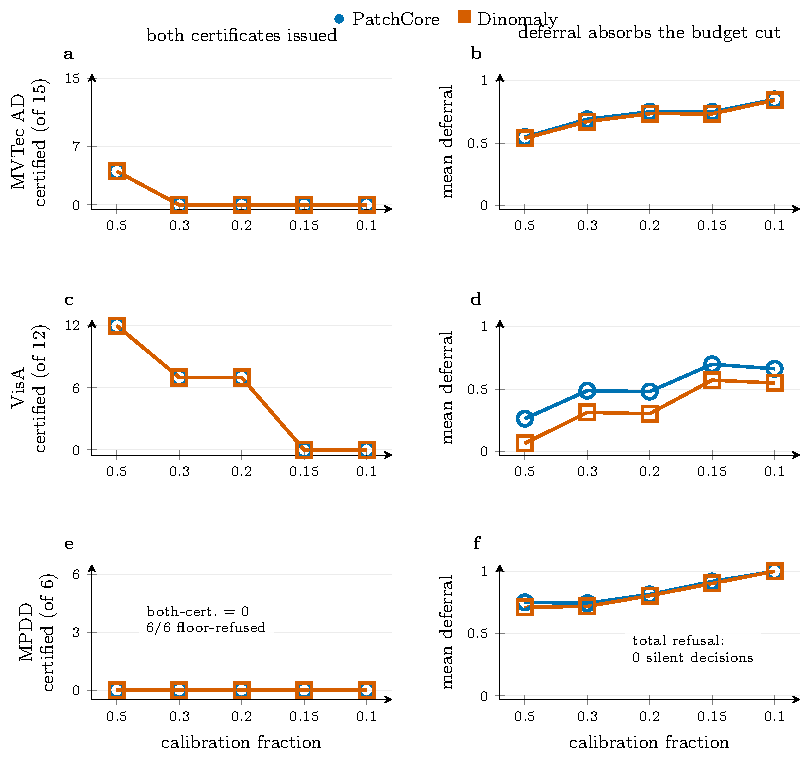
\includegraphics[width=\linewidth]{figures/fig-calfraction.pdf}
\caption{Calibration-budget sensitivity at the paper's operating point
($\alpha_{\text{miss}}=0.10$, $\alpha_{\text{fr}}=0.05$; $R=20$, five seeds;
post-freeze exploratory). Rows are MVTec AD (a,b), VisA (c,d), and MPDD (e,f).
Left panels show categories certified on both axes as the calibration fraction shrinks;
right panels show mean deferral. Shaded bands span seed minima to maxima. Lost budget
is absorbed by deferral, never by silent error: at fraction $0.10$ MPDD refuses
everything (deferral exactly $1.0$, zero silent decisions). The flat zero in panel (e)
for MPDD at fraction $0.10$ is a measured refusal across all $20$ repeats and five
seeds --- the floors refuse all six categories, so both-certified is identically zero
and deferral saturates at $1.0$ rather than crossing into silent mis-coverage.}
\label{fig:calfraction}
\end{figure}

A second deployment question the single-point headline leaves open is how much
calibration data the gate needs. We re-run the frozen protocol at the paper's operating
point while shrinking the calibration half of each split from $50\%$ to $10\%$ of the
test set (Figure~\ref{fig:calfraction}; post-freeze exploratory, same byte-identical
code path, verified against the frozen artifacts at fraction $0.50$). Three readings.
First, validity is budget-invariant: the mean pooled realized escaped-defect rate stays
at or below $\alpha_{\text{miss}}=0.10$ and the mean pooled false-reject rate at or below
$\alpha_{\text{fr}}=0.05$ at \emph{every} fraction, on every benchmark, for both
backbones (worst mean: escaped $0.095$, false-reject $0.039$); individual repeats on
small pools exceed the targets (worst single repeat: escaped $0.25$ on MPDD's
$\sim$14-defective cells), the expected finite-$n$ fluctuation of a marginal guarantee,
not a validity breach. Second, certification collapses exactly where the floor arithmetic
predicts: VisA's both-axis certification holds $12/12$ down to fraction $0.30$--$0.20$
and falls to $0$ at $0.15$ as per-category calibration pools cross below the
$1/(n_{\text{cal}}+1)$ floors; MVTec AD's four G2-certified categories are lost already
at fraction $0.30$ (its good pools are the smaller pools), while its G1 side degrades
gracefully $15\to8$ of $15$ at fraction $0.10$. Third, the degradation is into deferral,
never into silent error --- at fraction $0.10$ MPDD defers $100\%$ of images on both
backbones, the loudest possible refusal, with zero uncertified automated decisions. The
practical reading for a plant: the $50/50$ split is not a requirement but a choice on a
smooth budget curve, and whatever budget is spent, the certificate semantics do not
degrade --- only the coverage does.
% source: calfraction_sweep_2026-07-19/{results.json,RESULTS.md} (post-freeze
% exploratory; 6/6 frozen-reproduction checks PASS, max abs diff 0.0 at frac 0.50)

\subsection{How much calibration data buys a certificate: a planning curve}
\label{sec:calplanning}

The budget sweep above answers what happens when calibration data is taken \emph{away}. A plant
scoping a deployment asks the inverse, and it is the more actionable question: given a target
rate, how many labelled calibration images must be collected before the gate will certify at
all? The floor $\alpha_{\min}=1/(n_{\text{cal}}+1)$ inverts exactly, so this has a closed-form
answer --- certifying rate $\alpha$ on a category requires
\begin{equation}
n_{\text{cal}} \;\geq\; \lceil 1/\alpha \rceil - 1,
\label{eq:planning}
\end{equation}
of the relevant class (defective for escaped-defect, good for false-reject), per category, over
and above whatever pool the detector itself was fitted on. Figure~\ref{fig:calplanning} turns
Equation~\eqref{eq:planning} into a procurement curve and prices the three benchmarks against it.
% Place the float immediately after its citation so the long "Three readings"
% paragraph cannot push it into a near-empty orphan page.
\begin{figure}[htbp]
  \centering
  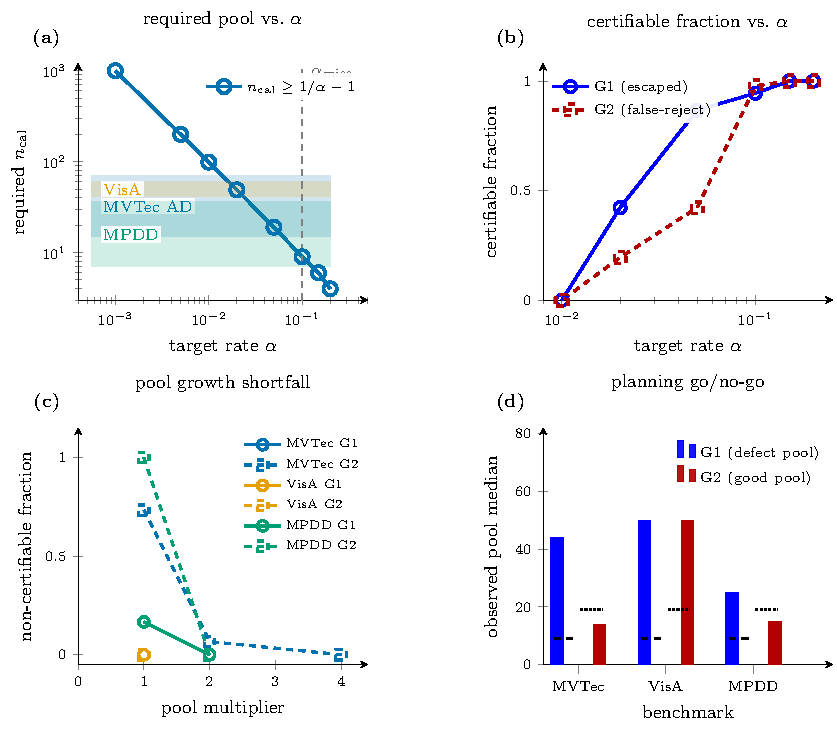
\includegraphics[width=\linewidth]{figures/fig-calplanning.pdf}
  \caption{Calibration-pool planning curves from the frozen per-category pool sizes.
  (a)~Required $n_{\text{cal}}$ vs.\ target rate $\alpha$ (Equation~\eqref{eq:planning}); shaded
  bands are observed defective-pool ranges, and the dashed line marks
  $\alpha_{\text{miss}}=0.10$. (b)~Certifiable category fraction vs.\ $\alpha$ (G1 escaped-defect,
  solid; G2 false-reject, dashed), averaged over both backbones. (c)~Pool-growth shortfall at the
  operating point as the \emph{non}-certifiable fraction (zero $=$ already fully certified).
  (d)~Go/no-go check: bars are observed median pool sizes; dashed segments are the required
  $n_{\text{cal}}$ on each axis.}
  \label{fig:calplanning}
\end{figure}
The arithmetic is analytic, but we verify it against the frozen artifacts: at the paper's
operating point it reproduces every frozen certified count exactly ($6/6$ benchmark $\times$
backbone checks, MVTec AD G1 $15/15$ / G2 $4/15$, VisA $12/12$ / $12/12$, MPDD $5/6$ / $0/6$).

Three readings, and the first reframes the paper's own refusals. The rates certified here are
\emph{cheap}: $\alpha_{\text{miss}}=0.10$ costs $9$ defective images per category and
$\alpha_{\text{fr}}=0.05$ costs $19$ good ones. Consequently the G2 refusals reported
throughout --- MPDD $0/6$, MVTec AD $11/15$ --- are not a deep obstruction but a shortfall of
roughly a factor of two in test-split allocation: holding the protocol fixed and only doubling
each category's good pool takes MPDD from certifying nothing to certifying \emph{all} six
categories, and MVTec AD from $4/15$ to $14/15$ (Figure~\ref{fig:calplanning}(b); $4\times$
completes MVTec AD at $15/15$). MPDD's per-category test-good pools are $26$--$32$ images,
about half of the $38$ that a $50/50$ split would need to clear $19$. Second, the
escaped-defect axis is already nearly paid for: MVTec AD and VisA clear the $\alpha_{\text{miss}}$
floor in every category as collected, and MPDD misses only connector, whose $14$ test-defective
images yield $n_{\text{cal}}^{\text{def}}=7<9$. Third, the expense is concentrated entirely in
the tight rates a safety-critical line would actually want: $\alpha=0.01$ requires $99$ per
category and $\alpha=0.001$ requires $999$, which is $5$--$50\times$ what any of these
benchmarks supply. That is the quantitative form of the scope boundary we state in
Section~\ref{sec:limitations}: on data of this scale the demonstrable object is the refusal
discipline, and reaching a $1\%$-escape certificate is a data-collection problem rather than a
methodological one. We state the planning rule in that form --- Equation~\eqref{eq:planning} is a
hard procurement requirement, not a tuning knob, precisely because falling below it produces a
refusal instead of a quietly weaker certificate.
% source: calplanning_2026-07-29/{results.json,RESULTS.md} (post-freeze exploratory,
% analytic from frozen pool sizes; 6/6 operating-point reproduction checks PASS)

\subsection{Comparison with a conformal single-threshold baseline}
\label{sec:crcbaseline}

The natural named baseline a reviewer would ask for is not a hand-picked straw man but the
single-threshold construction our own G1 certificate specializes: split-conformal Conformal Risk
Control (CRC)~\citep{angelopoulos2022crc}, applied with one per-category threshold at
$\alpha_{\text{miss}}=0.10$ and no defer option. For the $0/1$ miss loss this threshold is exactly
our G1 split-conformal threshold (an identity proved in the gate module's implementation), so CRC and our gate
share the same finite-sample escaped-defect guarantee and certify the same cells; the only degree
of freedom is what each does with the ambiguous middle. We recompute CRC on the identical
canonical score dumps, under the identical protocol ($\alpha_{\text{miss}}=0.10$,
$\alpha_{\text{fr}}=0.05$, $R=20$ repeated stratified $50/50$ calibration/evaluation splits, five
seeds, both backbones), so every cell in Table~\ref{tab:crcbaseline} is apples-to-apples with the
main results. The pooled rate comparison uses Equation~\eqref{eq:crcrates}. CRC has no mechanism
to certify the false-reject side at all --- with one threshold, every non-passed image is an
auto-reject, not a deferral --- so its G2 column is structurally n/a.
\begin{equation}
\begin{aligned}
\widehat r_{\text{miss}}(m)
&=\frac{\sum_{i\in\mathcal P}\mathbf{1}\{y_i=\text{defective}\}
\,\mathbf{1}\{D_m(s_i;c_i)=\text{pass}\}}
{\sum_{i\in\mathcal P}\mathbf{1}\{y_i=\text{defective}\}},\\[2pt]
\widehat r_{\text{fr}}(m)
&=\frac{\sum_{i\in\mathcal P}\mathbf{1}\{y_i=\text{good}\}
\,\mathbf{1}\{D_m(s_i;c_i)=\text{reject}\}}
{\sum_{i\in\mathcal P}\mathbf{1}\{y_i=\text{good}\}},\\[2pt]
\widehat r_{\text{def}}(m)
&=\frac{1}{|\mathcal P|}\sum_{i\in\mathcal P}\mathbf{1}\{D_m(s_i;c_i)=\text{defer}\}.
\end{aligned}
\label{eq:crcrates}
\end{equation}
% source: baseline_comparison_2026-07-15/{results.json,RESULTS.md,runner.py}

\begin{table}[htbp]
  \centering
  \small
  \caption{Our dual gate vs.\ a single-threshold CRC baseline controlling the same escaped-defect
  risk ($\alpha_{\text{miss}}=0.10$), pooled over both backbones, five seeds, and all categories
  ($n_{\text{cells}} = 2\times5\times n_{\text{categories}}$ per benchmark). CRC certifies the same
  escaped-defect cells (G1) but has no false-reject certificate (G2 n/a) and must auto-reject the
  entire ambiguous band instead of deferring it.}
  \label{tab:crcbaseline}
  % source: baseline_comparison_2026-07-15/results.json (crc_baseline vs our_gate_published, pooled)
  \resizebox{\linewidth}{!}{%
  \begin{tabular}{@{}llccccc@{}}
    \toprule
    Benchmark & Method & G1 cert. & G2 cert. & Escaped & False-reject & Deferral \\
    \midrule
    MPDD     & Our dual gate     & 50/60   & 0/60    & $6.6\%$ & $0.0\%$  & $73.1\%$ \\
    MPDD     & CRC (single thr.) & 50/60   & n/a     & $6.6\%$ & $36.9\%$ & $0.0\%$  \\
    \addlinespace
    VisA     & Our dual gate     & 120/120 & 120/120 & $7.6\%$ & $3.0\%$  & $16.4\%$ \\
    VisA     & CRC (single thr.) & 120/120 & n/a     & $9.5\%$ & $16.2\%$ & $0.0\%$  \\
    \addlinespace
    MVTec AD & Our dual gate     & 150/150 & 40/150  & $7.3\%$ & $0.5\%$  & $54.4\%$ \\
    MVTec AD & CRC (single thr.) & 150/150 & n/a     & $8.5\%$ & $3.1\%$  & $0.0\%$  \\
    \bottomrule
  \end{tabular}%
  }
\end{table}
\FloatBarrier

On MPDD, where the false-reject floor refuses G2 entirely (Section~\ref{sec:floors}), the contrast
is starkest: CRC pays $36.9\%$ false-reject to hold the same $6.6\%$ escaped-defect rate our gate
holds at $0.0\%$ false-reject, by deferring $73.1\%$ of images instead of auto-rejecting them ---
and that $0.0\%$ is not a dual-certificate win, because G2 is refused in every MPDD category under
the primary protocol. VisA and MVTec AD show the same \emph{direction} at smaller magnitude
($16.2\%$ vs.\ $3.0\%$ false-reject on VisA; $3.1\%$ vs.\ $0.5\%$ on MVTec AD), but not equal
escaped-defect protection: CRC's realized escaped-defect rate is somewhat higher on these two
benchmarks ($9.5\%$ vs.\ $7.6\%$ on VisA, $8.5\%$ vs.\ $7.3\%$ on MVTec AD). The crossed-threshold
mechanism explains the gap without claiming bit-identical routes --- both methods control the same
nominal $\alpha_{\text{miss}}$ risk, yet CRC collapses the ambiguous middle into auto-reject while
the dual gate splits that mass into a certified reject band plus deferral --- so realized rates
differ within sampling noise across repeats. The comparison isolates exactly what the dual-gate
design buys over the nearest published single-threshold alternative: not a better escaped-defect
guarantee (both share the same conformal construction) but a false-reject guarantee CRC cannot
offer, purchased by turning auto-rejects into deferrals.
Figure~\ref{fig:crcbaseline} plots the three rates for both methods side by side across all three
benchmarks, making the MPDD contrast in particular immediately visible. A per-backbone breakdown
(Appendix Table~\ref{tab:crcbackbone}) confirms the pooled contrast is not carried by one
backbone, and exposes that CRC's VisA false-reject is itself strongly backbone-dependent
($28.8\%$ PatchCore vs.\ $3.7\%$ Dinomaly) --- the dual gate's deferral mechanism matters most
exactly where the detector underneath is weakest.

\begin{figure}[htbp]
  \centering
  % Panels a-d generated by R/process_crcbaseline.R -> out/crcbaseline-panel-*.tex,
  % rendered via tikz/fig-crcbaseline.tex (R/CSV/TikZ pipeline).
  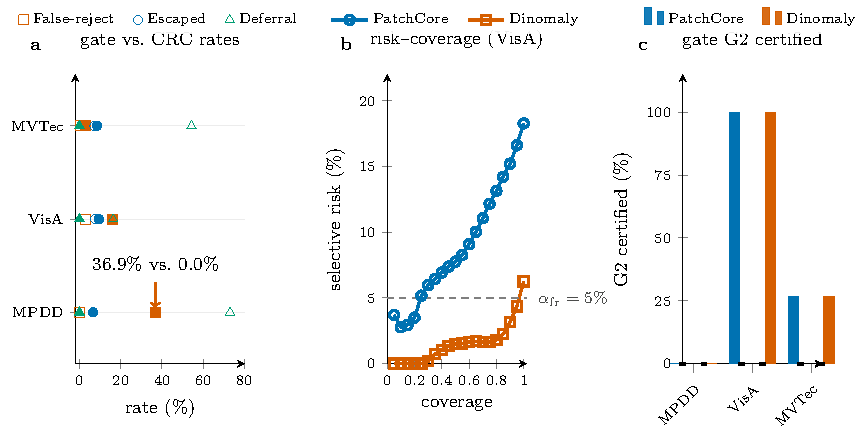
\includegraphics[width=\linewidth]{figures/fig-crcbaseline.pdf}
  \caption{Dual gate versus single-threshold CRC baseline, pooled over both backbones and five seeds
  (Table~\ref{tab:crcbaseline}). \textbf{a:} Escaped-defect, false-reject, and deferral rates
  side by side across all three benchmarks. CRC has no deferral mechanism, so every non-passed
  image becomes an auto-reject; on MPDD this drives its false-reject rate to $36.9\%$ against
  $0.0\%$ for our gate at the same escaped-defect rate. \textbf{b:} Selective-prediction
  risk-at-coverage curves per backbone on VisA --- the CRC baseline specializes to per-category
  selective classification with confidence-based abstention, but no coverage level reaches the
  $5\%$ false-reject guarantee the gate certifies. \textbf{c:} Per-backbone G2 certification:
  the gate certifies both backbones on VisA (60/60 cells each), one on MVTec AD (20/75 each),
  and neither on MPDD (0/30 each); CRC certifies zero cells on every benchmark and backbone
  (0/75 MVTec AD, 0/60 VisA, 0/30 MPDD, per backbone) --- it cannot deliver the
  false-reject guarantee at any coverage.}
  \label{fig:crcbaseline}
\end{figure}
\FloatBarrier

As a second, non-conformal reference line we also compute the field-standard selective-prediction
risk-coverage curve~\citep{geifman2017selective} (per-category best-F1 threshold, margin-based
abstention) on the same score dumps. Its area-under-the-risk-coverage-curve (AURC, lower is
better) ranges from $0.0019$ (MVTec AD, Dinomaly) to $0.0849$ (VisA, PatchCore); at $\sim\!80\%$
coverage the realized risk is $0.0625$/$0.0154$ (MPDD, PatchCore/Dinomaly), $0.1315$/$0.0180$
(VisA, PatchCore/Dinomaly), and $0.0095$/$0.0026$ (MVTec AD, PatchCore/Dinomaly). This is a
fundamentally different guarantee --- a curve traced out by sweeping coverage post hoc, not a fixed
pre-specified certificate at a chosen risk level --- so we report it as context rather than a
like-for-like comparison to Table~\ref{tab:crcbaseline}.
% source: baseline_comparison_2026-07-15/results.json (selective_baseline, per-backbone aurc + risk_at_coverage[coverage=0.8])

\subsection{Deployment cost analysis}
\label{sec:opcost}

Table~\ref{tab:crcbaseline} certifies the dual gate's rates but not their economic
consequence: every deferral is a decision routed to a human reviewer, and every
false-reject the gate avoids is one the CRC baseline pays for instead. We translate
both operating points into practitioner economics under three ASSUMED, explicitly
labeled illustrative deployment scenarios spanning a $30\times$ throughput range --- a
low-volume precision line ($100$ parts/hour, $\$5{,}000$ per escaped defect, $\$150$
per false reject, a $\$45$/hour reviewer at $120$ parts/hour), a mid-volume general
industrial line ($600$/hour, $\$300$/$\$15$, a $\$30$/hour reviewer at $240$/hour), and
a high-volume commodity line ($3{,}000$/hour, $\$25$/$\$2$, a $\$26$/hour reviewer at
$450$/hour) --- applied to the certified rates of Table~\ref{tab:crcbaseline} (neither
the rates nor the frozen calibration are altered; only the dollar figures are
scenario-dependent). The full nine-cell benchmark $\times$ scenario grid and script are
in the released artifact set of the code-and-data deposit; Table~\ref{tab:opcost}
shows the mid-volume scenario.
% source: opcost_analysis_2026-07-16/{script.py,results.json,RESULTS.md} (downstream cost-model transform of baseline_comparison_2026-07-15/results.json; no frozen number altered)

\begin{table}[htbp]
  \centering
  \small
  \caption{Deployment cost analysis, mid-volume general industrial scenario ($600$
  parts/hour, $\$300$ per escaped defect, $\$15$ per false reject, $\$0.125$/part
  review labor). Reviewer load is throughput $\times$ deferral rate; CRC's is $0$ by
  construction (no deferral mechanism --- every non-passed item is an automatic
  reject, not a human decision). Breakeven review cost/part is the human-review unit
  cost above which CRC would become cheaper than the dual gate, holding this
  scenario's other costs fixed; headroom is that breakeven divided by the
  $\$0.125$/part assumed here. The all-human row is a labor-only comparator
  ($\$30$/hour at $240$ parts/hour); no human miss/false-reject model is available, so its
  $\$75$/hour is not a like-for-like total-error-cost estimate.}
  \label{tab:opcost}
  % source: opcost_analysis_2026-07-16/results.json (benchmark_scenario_grid.*.mid_volume_general, breakeven_false_reject_cost_usd.*.mid_volume_general)
  \resizebox{\linewidth}{!}{%
  \begin{tabular}{@{}lccccc@{}}
    \toprule
    Benchmark / policy & Reviewer load & Gate/policy \$/hr & CRC \$/hr & Gate savings & Headroom \\
    \midrule
    MPDD     & $438.5$/hr ($1.83$ FTE) & $\$11{,}990$ & $\$15{,}252$ & $+\$3{,}262$/hr & $61\times$  \\
    VisA     & $98.4$/hr ($0.41$ FTE)  & $\$14{,}024$ & $\$18{,}547$ & $+\$4{,}522$/hr & $369\times$ \\
    MVTec AD & $326.1$/hr ($1.36$ FTE) & $\$13{,}134$ & $\$15{,}661$ & $+\$2{,}527$/hr & $63\times$  \\
    All-human baseline & $600.0$/hr ($2.50$ FTE) & $\$75$ labor only & --- & --- & --- \\
    \bottomrule
  \end{tabular}%
  }
\end{table}
\FloatBarrier

The all-human row exposes the labor floor behind the scenario: reviewing all $600$ parts/hour at
$240$ parts/hour per reviewer requires $2.50$ FTE and costs $\$75$/hour. It is deliberately
labor-only because the frozen artifacts contain no human miss or false-reject model; it therefore
contextualizes staffing, not comparative decision quality.

The dual gate is cheaper than CRC in all nine benchmark $\times$ scenario
combinations we compute, though the economic case varies by deferral cost. On VisA and MVTec AD, where
deferral rates are moderate ($16.4\%$ and $54.4\%$ respectively), the gate saves $\$2{,}527$--$\$4{,}522$/hour
at mid-volume with substantial headroom ($63$--$369\times$). MPDD is economically viable only in scenarios
where high review capacity is available or tolerable: at mid-volume its $73.1\%$ deferral translates to
$438.5$ parts/hour ($1.83$ FTE), saving $\$3{,}262$/hour against CRC\'s $36.9\%$ false-reject rate, but
at high-volume the same deferral becomes $2{,}192.7$ parts/hour (nearly five FTEs) --- positioning MPDD
as a high-review diagnostic scenario rather than a universally economical deployment. The saving is not an artifact of favorable escaped-defect
rates: on MPDD the two methods share the identical escaped-defect rate by the proven
G1$\equiv$CRC threshold identity, and on VisA/MVTec AD the gate's escaped rate is
additionally somewhat \emph{lower} than CRC's. The least robust cell is MVTec AD under
the high-volume commodity scenario: human review would need to cost more than
$\$0.69$/part before CRC becomes cheaper there, about $12\times$ the $\$0.058$/part
assumed in that scenario. Every other cell has $17$--$1{,}833\times$ headroom. This
model omits reviewer error rate, queueing dynamics, and an appeal channel for CRC's
false-rejected good parts; modeling the latter would raise CRC's cost further, so the
comparison is if anything conservative toward CRC. Its dollar figures are
scenario-dependent by construction, while the throughput-invariant breakeven
quantities above are the assumption-robust takeaway.

Figure~\ref{fig:opcost} shows the deployment economics of the certified gate versus the CRC baseline.
\begin{figure}[htbp]
\centering
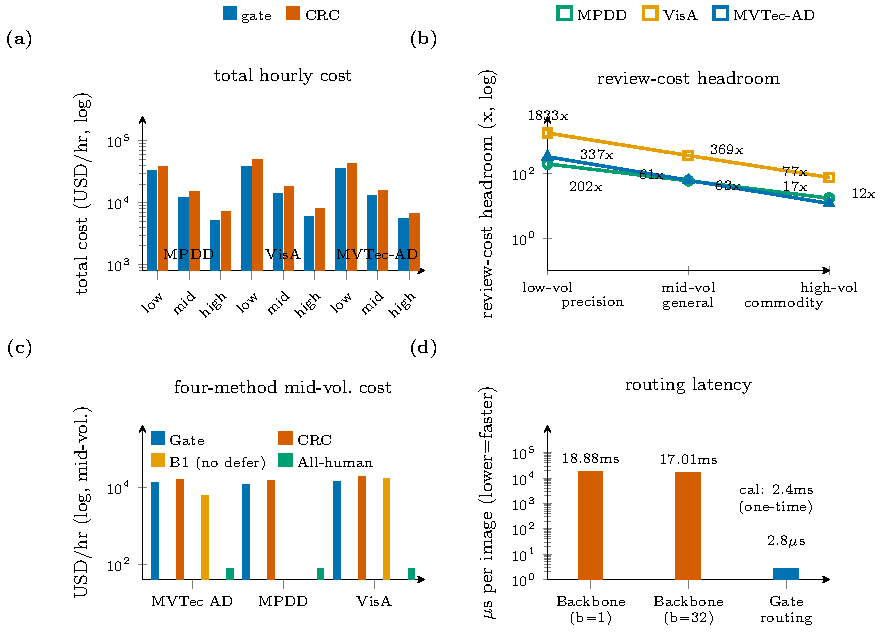
\includegraphics[width=\linewidth]{figures/fig-opcost.pdf}
\caption{Deployment economics of the certified gate versus the CRC single-threshold
baseline at frozen rates. Scenario groups: low-volume precision ($100$ parts/hour),
mid-volume general ($600$), high-volume commodity ($3{,}000$); scenarios are assumed
illustrative inputs. \textbf{a:}~Total hourly cost (gate vs.\ CRC) across all nine
benchmark--scenario cells: the gate is cheaper in every cell. \textbf{b:}~Review-cost
headroom --- the multiple by which the assumed review cost can rise before the gate stops
being cheaper: $12\times$--$1833\times$ (log; break-even at $1\times$). \textbf{c:}~Four-method
total hourly cost at mid-volume general, including the original B1 binding-demo arm (no
deferral, post-hoc, unavailable for MPDD); the gate is cheapest on MVTec AD and VisA.
\textbf{d:}~Routing latency: the gate adds $2.8\,\mu$s per image amortised (right bar),
against $18.9\,$ms backbone inference at batch size 1 and $17.0\,$ms batched (left bars).
Calibration is a one-time $2.4\,$ms per reset.}
\label{fig:opcost}
\end{figure}


\subsection{Latency and deployment cost}
\label{sec:latency}

The gate is a thin decision layer on top of whatever detector already produces the anomaly score,
so the only cost it adds is the conformal calibration (once, per calibration refresh) and the
per-image routing comparison. We measured both on this work's hardware, and we place them
alongside the backbone forward pass that dominates the end-to-end budget
(Table~\ref{tab:latency}). Routing an image is an $O(1)$ threshold comparison inside an
$O(\text{sort})$ calibration; the measured per-image routing cost is $2.8\,\mu$s on CPU ---
roughly four orders of magnitude below the backbone forward pass and under $0.02\%$ of Dinomaly's
per-image GPU inference. Calibrating the full three-way gate over one $861$-image calibration half
across all $15$ MVTec strata (the $\alpha_{\text{miss}}=0.10$, $\alpha_{\text{fr}}=0.05$ primary
configuration) takes $2.4$ ms end to end, and is amortized over an entire evaluation run rather
than paid per image. The practical conclusion is that certification is free relative to detection:
a deployment already able to afford the detector can add the escaped-defect / false-reject
certificate at no measurable latency cost. The backbone rows are the honest budget the gate sits
on --- Dinomaly measured here on an RTX~5090 Laptop GPU, PatchCore's row taken from the authors'
reported figure (not measured here, and both hardware- and coreset-dependent). We flag the
substrate mix these numbers span, so no cross-row comparison is over-read: the gate rows are timed
on CPU over the MVTec calibration scores ($861$-image cal half, $15$ strata), the Dinomaly backbone
row on GPU over $250$ real VisA test images (the VisA branch-A seed-$0$ checkpoint), and the
PatchCore row is the authors' published $\sim$1\%-coreset figure whereas our scoring uses the
$10\%$-coreset configuration --- so the table brackets the order of magnitude of the
backbone budget the gate rides on, and it is the $\mu$s-scale CPU gate overhead, not any
CPU-vs-GPU or MVTec-vs-VisA backbone comparison, that the paper contributes.
% source: latency_2026-07-13/gate_latency.json (gate rows, measured CPU;
% Intel Core Ultra 9 275HX / 24 threads / 62 GB);
% latency_2026-07-13/dinomaly_latency.json (Dinomaly row, measured RTX 5090 Laptop GPU,
% torch 2.12.0+cu130, VisA branch-A seed-0 checkpoint, 250 real VisA test images);
% PatchCore row attributed to Roth et al. 2022 (published, not measured).
% KEEP (directive #2 remedy d): checked gate_latency.json/dinomaly_latency.json for
% per-category/per-seed rows to expand into -- none exist beyond these 2 single-point gate
% measurements (calibrate/route) and 2 backbone figures; this is the full granularity the
% frozen measurements support, so the 4-row table is load-bearing as-is (no merge partner
% exists either -- no other latency table in the paper).

\begin{table}[htbp]
  \centering
  \small
  \caption{Per-image latency and deployment cost. The two gate rows and the Dinomaly backbone row
  are \emph{measured on this work's hardware} (gate: Intel Core Ultra~9 275HX CPU, $24$ threads;
  Dinomaly: NVIDIA RTX~5090 Laptop GPU, torch~2.12.0, batch~$1$, median over $250$ real VisA test
  images, full forward\,$+$\,anomaly-map\,$+$\,image-score pass). The PatchCore backbone row is
  \emph{reported by the authors} (not measured here; Roth et al.~\citep{roth2022patchcore}, $\sim$1\%-coreset
  configuration on their hardware) and is included only to bracket the backbone budget --- backbone
  timing is hardware- and configuration-dependent, whereas the gate overhead below it is the
  measured constant this paper contributes. Sources: the frozen latency measurement dumps.}
  % source: latency_2026-07-13/{gate,dinomaly}_latency.json
  \label{tab:latency}
  \small
  \begin{tabular}{@{}>{\raggedright\arraybackslash}p{0.34\textwidth} l >{\raggedright\arraybackslash}p{0.34\textwidth}@{}}
    \toprule
    Component & Per-image cost & Notes \\
    \midrule
    \multicolumn{3}{@{}l}{\emph{Backbone forward pass (dominates the budget)}} \\
    \quad Dinomaly (DINOv2-b, $148$M) --- measured, GPU & $18.9$ ms (p95 $23.1$) & $53$ img/s at batch $1$; $17.0$ ms/img batched ($B{=}32$) \\
    \quad PatchCore (WRN50, coreset) --- \emph{authors' figure} & $\lesssim 200$ ms & Roth et al.~\citep{roth2022patchcore}, their hardware; not measured here \\
    \midrule
    \multicolumn{3}{@{}l}{\emph{Gate overhead added on top (this paper) --- measured, CPU}} \\
    \quad Routing (per image) & $2.8\,\mu$s & $O(1)$ compare; $<0.02\%$ of the Dinomaly forward pass \\
    \quad Calibration (one-time) & $2.4$ ms (p95 $2.8$) & full $3$-way gate, $861$-img cal half, $15$ strata; per refresh \\
    \bottomrule
  \end{tabular}
\end{table}
\FloatBarrier


\subsection{G2 train-holdout promotion on MVTec AD (frozen remedy arm)}
\label{sec:g2promo}

The preregistered calibration-efficiency remedy --- recalibrating G2 on held-out
\emph{train}-good scores, gated behind a per-category Kolmogorov--Smirnov (KS) exchangeability test with a mandatory
audited-not-certified fallback --- was computed after the freeze,
for PatchCore only: post-freeze MVTec/VisA Dinomaly train-score dumps now exist, but they are
checkpoint-dependent and do not provide the independent held-out pool required for a fresh G2
promotion calibration. The remedy arm therefore remains single-backbone by evidence eligibility,
disclosed here rather than implied otherwise. It behaves as preregistered: G2-certifiable categories rise from
$4/15$ to $13/15$ in seeds $0$--$3$ and $12/15$ in seed $4$. The KS gate does real work rather than rubber-stamping:
leather fails it in all five seeds (its train-good and test-good score distributions are not
exchangeable) and screw additionally fails in seed $4$ --- each is reported
audited-not-certified, never silently promoted, and the seed-$4$ screw case shows a category
certified under the primary protocol can still be \emph{refused} under the holdout arm when
exchangeability breaks. Toothbrush remains uncertifiable at $\alpha_{\text{fr}}=0.05$ under both
arms, exactly as preregistered ($n^{\text{good}}$ too small in either pool). K1 is not tripped
in any promoted seed aggregate.

\paragraph{What the remedy costs and delivers (post-freeze pricing).} Figure~\ref{fig:g2delta} shows the per-category certification flip.

\begin{figure}[htbp]
\centering
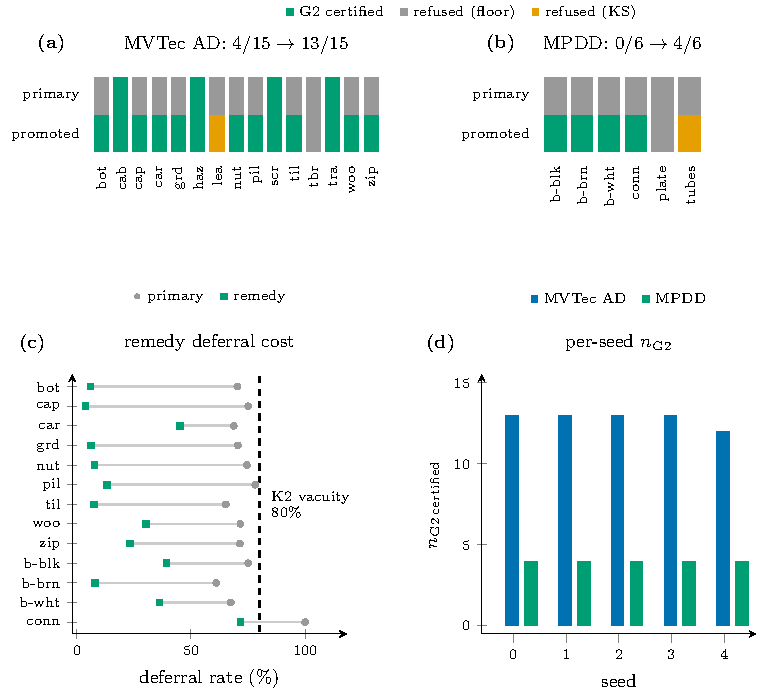
\includegraphics[width=0.95\linewidth]{figures/fig-g2delta.pdf}
\caption{The G2 train-holdout remedy (PatchCore; seeds $0$--$3$ identical, seed $4$ differs on
screw). \textbf{a:}~MVTec AD: $4/15\to13/15$, leather KS-refused every seed.
\textbf{b:}~MPDD: $0/6\to4/6$. Category codes --- MVTec AD: bot/cab/cap/car/grd/haz/lea/nut/pil/scr/til/tbr/tra/woo/zip;
MPDD: b-blk/b-brn/b-wht/conn/plate/tubes. Tiles: certified (green), refused at floor (grey), refused by KS (amber).
\textbf{c:}~Remedy deferral cost per rescued category: promotion opens the auto-reject region and
\emph{reduces} deferral for most categories; connector (MPDD) remains near-vacuous at $71.7\%$.
\textbf{d:}~Per-seed $n_{\mathrm{G2\,certified}}$ under the promoted arm: $13/15$ stable in seeds
$0$--$3$ (screw degrades to $12/15$ in seed $4$ when KS fails); MPDD holdout certifies $4/6$ in
all five seeds.}
\label{fig:g2delta}
\end{figure}

Pricing the flip on the
frozen post-hoc remedy-pricing artifacts qualifies it in both directions. On the cost
side, certification is \emph{not} bought with more deferral: opening the auto-reject region
(a finite $t_{\text{hi}}$ where the primary protocol refused) \emph{reduces} deferral in every
rescued category --- capsule certifies at $3.9\%$ mean deferral (from $75.1\%$ under refusal),
bottle $6.1\%$, tile $7.5\%$, metal\_nut $7.7\%$; the most expensive rescue is carpet at
$45.2\%$. On the honesty side, two flags travel with the headline. First, the already-certified
screw \emph{degrades} under the promotion arm: its realized false-reject mean rises to $8.8\%$
(range $4.8$--$12.1\%$ across seeds, above the $5\%$ target in four of five seeds and above the
$+3$\,pp tier-1 tolerance in three) before it KS-fails outright in seed $4$ --- the $13/15$
figure is therefore strictly a seeds-$0$--$3$ statement, and the promotion arm is a per-category
choice, not a global upgrade. Second, grid, zipper, and pill realize false-reject marginally
above the $5\%$ point target in some seeds (max $6.8\%$/$5.6\%$/$7.7\%$ respectively) though
always inside the tier-1 tolerance. G1 is structurally unaffected by the arm; every rescued
category's realized escaped-defect rate stays within target plus tolerance in every seed.
% source: frozen post-hoc remedy-pricing artifacts (results and summary; post-freeze exploratory)
% source: g2_promotion_2026-07-12/G2-PROMOTION-RESULT.json (summary + compare);
% SIGN-OFF-RECORD-2026-07-11.md (freeze); PREREG-DRAFT-2026-07-10.md §3.1/§8

\subsection{MPDD train-holdout rescue (post-freeze exploratory)}
\label{sec:mpddholdout}

We report the primary-protocol $0/6$ of the preceding section as MPDD's thesis-confirming
headline; the train-holdout arm below is a clearly secondary, post-freeze, PatchCore-only result.
The train-holdout calibration-efficiency lever the frozen MVTec remedy exercises
(Section~\ref{sec:g2promo}) turns MPDD's $0/6$ primary refusal into a $4/6$ rescue, a vivid
single-benchmark illustration of the same lever. MPDD's train-good pools are large ($54$--$289$ per category) where its
test-good pools are tiny, so recalibrating G2 on a $20\%$ held-out train-good pool (the flag-gated
train-holdout calibration mode, $20\%$ holdout fraction; PatchCore only, as on
MVTec --- MPDD has no Dinomaly train-score dump, while the later MVTec/VisA dumps are
checkpoint-dependent and not eligible independent holdouts for this arm)
clears the false-reject floor for the $5/6$ categories whose holdout pool reaches $n\ge 19$. The
same per-category KS exchangeability gate then adjudicates each promotion, and it does decisive
work: G2-certifiable rises from $0/6$ to $4/6$, identical in all five seeds. Two
categories are honestly held back --- metal plate, whose holdout pool ($11$) is still
below the floor, and tubes, which fails the KS gate (Benjamini--Hochberg (BH)-adjusted $p\approx
1.2\times10^{-5}$; its train-good and test-good score distributions are demonstrably
non-exchangeable) and is reported audited-not-certified rather than promoted. The remaining four
(bracket black, bracket brown, bracket white, connector)
promote cleanly (KS $p_{\text{BH}}\ge 0.44$ every seed). Connector is the one category
G1 refuses under the primary protocol ($n_{\text{cal}}^{\text{def}}=7<9$ defective) yet
the arm G2-certifies (holdout-good $26\ge 19$): the two certificates gate on independent sample
axes --- defect count for escaped-defect, good count for false-reject --- so this is coherent, not
contradictory. Even certified, connector still defers $71.7\%$ of all images under the arm
(down from $100\%$ under refusal; G1's empty auto-pass region caps what G2 alone can recover),
so that certificate remains operationally near-vacuous. The cheapest rescue is bracket brown at
$8.1\%$ mean deferral with realized false-reject $0.0\%$ in every seed; the one realized-rate
flag is bracket black, whose per-seed false-reject hits $10.0\%$ in two of five seeds (mean
$5.1\%$) --- the certificate bounds the \emph{expected} rate at $5\%$, but the realized rate is
seed-unstable there, and a deployment should treat the category as marginal. So the count-only
floor of $5/6$ is
audited down to a genuinely certified $4/6$ --- the KS guardrail keeping the rescue honest, exactly
the exchangeability risk MPDD's non-homogeneous backgrounds were expected to pose. As a sanity
check (no gate), the holdout arm's $80\%$-memory-bank test scores rank-correlate with the primary
$100\%$-bank scores at Spearman $\rho\ge 0.918$ across all $6\times5$ category-seed cells (max
$|\Delta\text{image-AUROC}|=0.040$), confirming the same model was scored. This arm is post-freeze
exploratory and flag-gated prereg-neutral (it re-freezes nothing and is never in the confirmatory
Holm family); the $0/6 \to 4/6$ contrast on the same benchmark and the same scores is a vivid
single-benchmark demonstration of the calibration-efficiency lever. The larger, \emph{confirmatory}
instance of the same lever is the frozen MVTec train-holdout remedy (Section~\ref{sec:g2promo}),
which lifts G2 from $4/15$ to $12$--$13/15$ across seeds ($13$ in seeds $0$--$3$, $12$ in seed~$4$).
The primary-protocol $0/6$ stays the honest headline for this industrial benchmark: on real metal
parts the gate certifies nothing at the $5\%$ false-reject budget because the data cannot pay for
it --- exactly what a refusal-first design should do.
% source: mpdd_results_2026-07-13/HOLDOUT-RESULTS.json (summary: g2_certified_by_seed=4 all seeds,
%   floor-only prediction 5/6, tubes KS p_bh 1.2e-5, metal_plate n=11<19, min Spearman 0.9186,
%   max|auroc_delta| 0.0399); run_mpdd_holdout_analysis.py

\subsection{When a fixed threshold over-promises (post-hoc binding demonstration)}
\label{sec:binding}

The excess-AURC audit of Section~\ref{sec:auditres} shows practice earns deferral skill, but it does not directly exhibit the
sharper event: a category where a \emph{naive fixed threshold} actually violates a target error
rate while the certified gate holds. We test that event directly, post-hoc. For each
(backbone, category) we take the naive practitioner's operating point --- a single global best-F1
threshold (B1) applied to every eval image with no deferral --- and compute its realized
escaped-defect and false-reject rates on the held-out eval half; alongside it we compute the
certified gate's realized rates and its deferral cost on the same split (mean over the $R=20$
repeats, at backbone seed $0$). A cell \emph{binds} when the fixed threshold's realized rate
exceeds the target ($\alpha_{\text{miss}}=0.10$ or $\alpha_{\text{fr}}=0.05$) while the gate's stays
within target$+3$pp.
% source: binding_demo_2026-07-13/results.json (per-cell B1 vs gate realized rates)

Such cells exist, on both benchmarks, both axes, and both backbones. Restricting to the strongest
evidence --- cells where the gate is certified on that axis in all $20$ repeats and the bind
holds in all five backbone seeds --- there are $27$: on MVTec AD, $3$ escaped-axis (Dinomaly on
capsule, pill, screw) and $3$ false-reject-axis (PatchCore on screw; Dinomaly on cable,
transistor); on VisA, $4$ escaped-axis and $17$ false-reject-axis cells. Crucially the effect is not
an artifact of the gate abstaining on everything: the cleanest cases pay a small deferral cost. On
MVTec AD a global threshold lets $24.2\%$ of defective screws escape; the certified gate,
deferring just $4\%$ of images, holds the escaped rate at $8.0\%$ (under target) because its
per-category (Mondrian) calibration puts the auto-pass boundary where a global threshold cannot. On
the false-reject axis, the same global threshold auto-rejects $19.5\%$ of good screws while the gate
holds false-reject at $5.0\%$ (certified, $14\%$ deferral); on VisA the extreme case is capsules,
where a global threshold would auto-reject $96.8\%$ of good parts and the gate holds false-reject at
$3.7\%$. The mechanism the demonstration exposes is that a single fixed \emph{global} threshold
cannot serve categories with different score scales at once, so it over-promises on whichever it
mis-fits; the certified gate refuses (defers) exactly where it cannot honor the target and
calibrates per category elsewhere. This is a post-hoc, exploratory illustration --- not a
preregistered arm --- and is reported verdict-honestly: had no cell bound, we would have kept the
``not demonstrated'' framing. Figure~\ref{fig:bindingesc} shows every escaped-defect-axis
binding cell: in each row the naive threshold sits beyond the target line while the certified
gate holds it, at the annotated deferral price.

\begin{figure}[htbp]
\centering
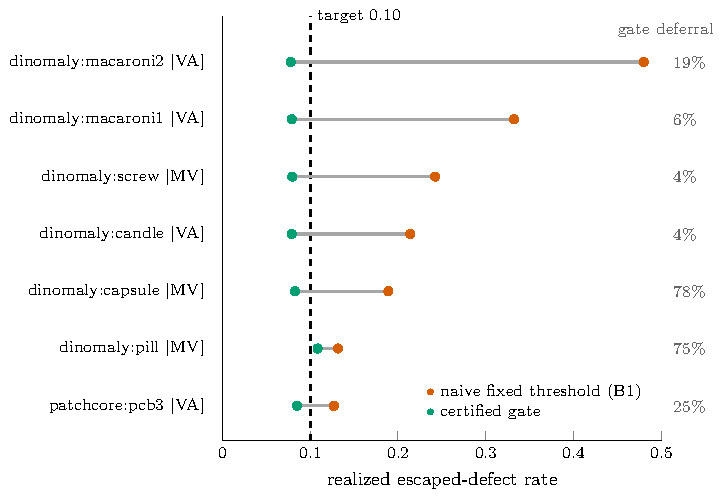
\includegraphics[width=\linewidth,height=0.42\textheight,keepaspectratio]{figures/fig-binding-escaped.pdf}
\caption{Binding cells on the escaped-defect axis (post-hoc). Per (backbone, category)
cell: realized escaped-defect rate of the naive global best-F1 threshold (vermillion)
vs.\ the certified gate (bluish green), with the gate's deferral annotated at right; the
dashed line is the $\alpha_{\text{miss}}=0.10$ target. MV $=$ MVTec AD, VA $=$ VisA.}
\label{fig:bindingesc}
\end{figure}
\FloatBarrier

Figure~\ref{fig:bindingfr} reports the corresponding false-reject binding cells under the same encoding.
\begin{figure}[htbp]
\centering
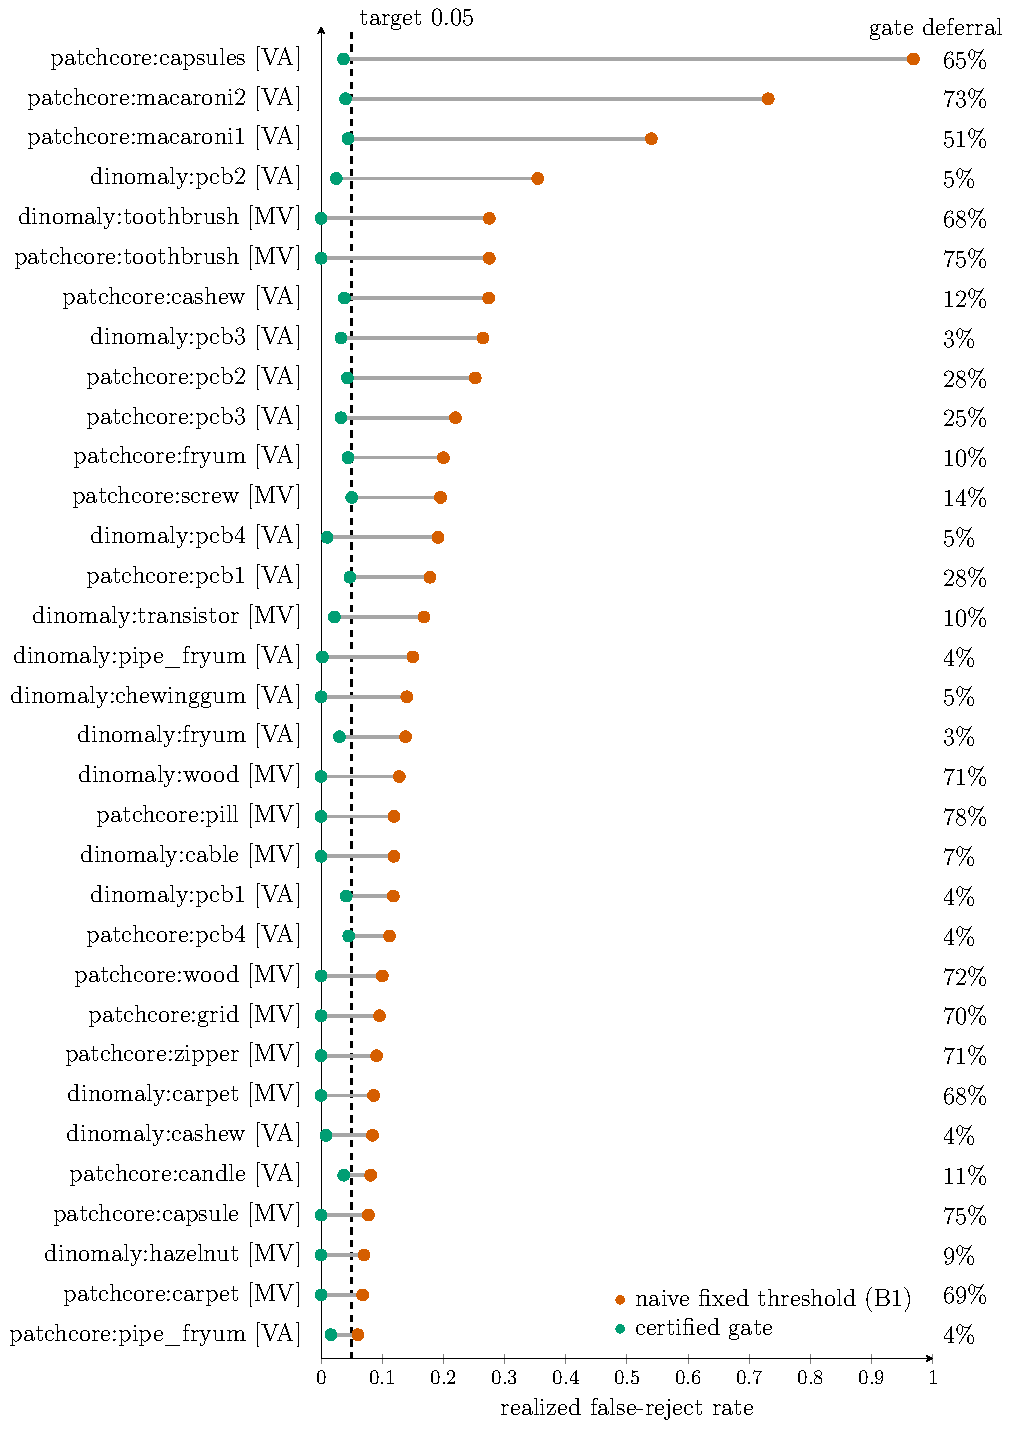
\includegraphics[width=\linewidth]{figures/fig-binding-fr.pdf}
\caption{Binding cells on the false-reject axis (post-hoc). Same encoding as
Figure~\ref{fig:bindingesc}; the dashed line is the $\alpha_{\text{fr}}=0.05$ target.
The VisA PatchCore capsules cell (top) is the extreme case: a global threshold
auto-rejects $96.8\%$ of good parts where the certified gate holds $3.7\%$.}
\label{fig:bindingfr}
\end{figure}


\subsection{Validity audit V1 (tier-1) and the kill-gates}
\label{sec:v1res}

Per frozen amendment A3, tier-1 is reported \emph{per axis}, with the false-reject axis
evaluated only over G2-certified cells: wherever G2 is refused the auto-reject region is empty
and the measured false-reject rate is identically $0$ --- a pass without evidence that A3
excludes from every count. On the escaped-defect axis, tier-1 passes in all $150$
MVTec cells ($2$ backbones $\times 5$ seeds $\times 15$ categories), all $120$
VisA cells ($2 \times 5 \times 12$), and all $60$ MPDD cells ($2 \times 5 \times 6$),
every rate within target$+3$pp. On the false-reject
axis, MVTec has $40$ evaluable cells ($4$ G2-certified categories $\times 2 \times 5$) and
passes $40/40$, with the other $110$ cells reported G2-REFUSED and excluded; on VisA
every category is G2-certified, so all $120/120$ cells are evaluable and pass
non-vacuously; on MPDD every category is G2-refused under the primary protocol, so all $60$
false-reject cells are G2-REFUSED and excluded (the mirror image of VisA, and the primary-protocol
counterpart to the train-holdout rescue of Section~\ref{sec:mpddholdout}). Tier-1 is a necessary-not-sufficient pipeline check --- a conservative gate
realizes rates well below target, so passing validates the calibrate/route/evaluate machinery
rather than demonstrating sharpness. Consequently K1 is not tripped (the A3 exclusion
cannot change K1's count: excluded cells cannot fail) ($0$ violations in every
(backbone, seed) aggregate, against the $5$-cell MVTec/VisA kill threshold and, on MPDD, against
a proportionally-scaled $2$-cell threshold\footnote{Absolute kill thresholds are un-trippable at
$n_{\text{cat}}=6$, so MPDD uses proportional scales (K1$\to 2$, K2$\to 4$); diagnostic only.}) and K2 is
not tripped (on MVTec/VisA at most $1$ vacuous category --- VisA/PatchCore/seed~$2$ --- against the
$8$-category/$0.80$-deferral threshold; on MPDD at most $2$ vacuous categories per aggregate
against the scaled $4$-category threshold), in all $30$ aggregates across the three
benchmarks (Table~\ref{tab:v1}). Table~\ref{tab:deferral} reports seed-$0$ median per-category deferral, its mean where computed,
and the extreme categories, for each benchmark and backbone. MVTec AD's deferral is elevated
because G2 refusal empties the auto-reject band in $11/15$ categories, though still far from the
vacuity threshold. VisA's deferral drops sharply because G2 certifies every category there, so the
auto-reject band is live throughout --- direct operational evidence that the elevated MVTec
deferral is the price of honest G2 refusal, not a property of the gate. MPDD sits at the far end:
G2 is refused in all $6$ categories under the primary protocol, exactly what $0/6$ certification
predicts. These are three honest operating points, not a defect and a fix: the elevated MVTec and
MPDD deferral is the cost of refusing to certify small good-calibration pools, and VisA's low
deferral is what the same gate, same code path, spends when the good pools are large enough to
certify every category.

The per-repeat validity audit is shown in Figure~\ref{fig:validity}.
\begin{figure}[tbp]
\centering
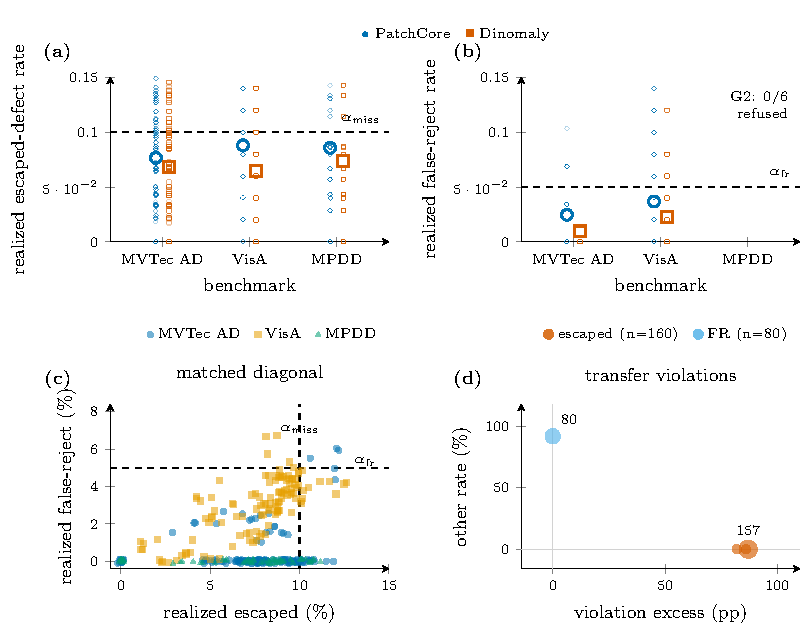
\includegraphics[width=\linewidth,height=0.52\textheight,keepaspectratio]{figures/fig-validity.pdf}
\caption{Per-repeat realized rates (frozen protocol; $6{,}400$ escaped-defect and $3{,}200$
false-reject certified-cell measurements). \textbf{a:}~Escaped-defect rate vs.\
$\alpha_{\text{miss}}=0.10$; \textbf{b:}~false-reject rate vs.\ $\alpha_{\text{fr}}=0.05$
(MPDD has no G2-certified cells under the primary protocol). Heavy dashes are per-(benchmark,
backbone) means; every mean sits below target. \textbf{c:}~Matched-diagonal validity cloud
($330$ cells, same-detector diagonal from the cross-detector transfer experiment): the
certified region sits at or below both targets, confirming the guarantee holds on the
same-detector reference. \textbf{d:}~Transfer violation cloud: $160$ escaped-defect
violations (transfer adds $82$--$87$ pp above $\alpha_{\text{miss}}$) and $80$ false-reject
violations; the two violation types separate cleanly by direction.}
\label{fig:validity}
\end{figure}

Figure~\ref{fig:validity} opens up the tier-1 aggregates above to the per-repeat level: the
certified clouds sit at or below target on the overwhelming majority of repeats, the
per-(benchmark, backbone) means sit below target everywhere, and the visible excursions are
single repeats on small cells --- the fluctuation the marginal certificate semantics predict,
not a validity breach (Section~\ref{sec:calfraction} shows the same invariance holds down to
a tenth of the calibration budget).

Figure~\ref{fig:deferral} shows median deferral per category for both backbones.
\begin{figure}[tbp]
\centering
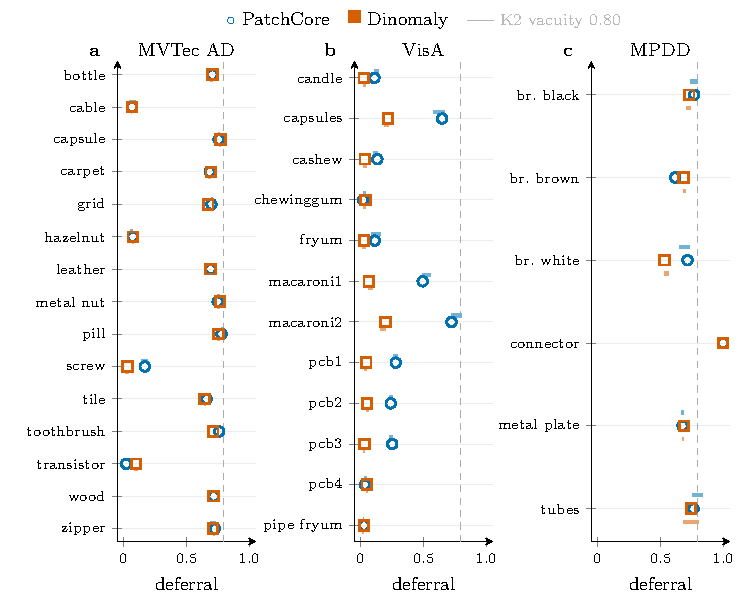
\includegraphics[width=\linewidth,height=0.48\textheight,keepaspectratio]{figures/fig-deferral.pdf}
\caption{Median deferral per category, seeds $0$--$4$ (dot = seed 0, shaded band = seed
$0$--$4$ min--max; $R=20$), both backbones. \textbf{a:}~MVTec AD. \textbf{b:}~VisA.
\textbf{c:}~MPDD. Deferral is strongly category-heterogeneous and tracks certifiability
(refused strata defer by construction). The K2 vacuity threshold ($0.80$, dashed) is
approached only on a handful of G2-refused categories; seed spread is narrow except
there.}
\label{fig:deferral}
\end{figure}
% source: analysis_2026-07-10/SUMMARY.json["gate_calibration_k1_k2"]; ANALYSIS-MEMO.md §3;
% visa_results_2026-07-12/SUMMARY.json["gate_calibration_k1_k2"] + gate_calibration/v1_*_seed0.json
% MPDD deferral: mpdd_results_2026-07-13/gate_calibration/v1_{patchcore,dinomaly}_seed0.json
%   ["median_deferral_by_category"]: patchcore median 0.7407->74.1%, min bracket_brown 0.6184->61.8%,
%   connector 1.0->100%; dinomaly median 0.7091->70.9%, min bracket_white 0.5333->53.3%, connector 1.0->100%

\begin{table}[htbp]
  \centering
  \caption{V1 tier-1 (per axis, per frozen amendment A3) and kill-gates, aggregated over the
  $30$ (backbone, seed) cells across all three benchmarks. $^{\dagger}$False-reject evaluated only
  over the $4$ G2-certified MVTec categories; the other $110$ cells are G2-REFUSED and excluded
  from the count, never counted as (vacuous) passes. $^{\ddagger}$On MPDD all $60$ false-reject
  cells are G2-REFUSED under the primary protocol and excluded (see Section~\ref{sec:mpddholdout}
  for the train-holdout rescue). MPDD's K1/K2 thresholds are proportionally scaled to $n_{\text{cat}}=6$
  ($2$ and $4$). ``---'' marks a cell that does not apply to that row (the raw evaluable-cell
  counts above have no separate threshold or trip verdict; K5 never fires under the frozen
  design, so it reports no single value). Sources: the frozen MVTec AD, VisA, and MPDD
  analysis summaries and their per-cell validity dumps; frozen preregistration \S9 amendment A3.}
  % source: analysis_2026-07-10, visa_results_2026-07-12, mpdd_results_2026-07-13
  % SUMMARY.json["gate_calibration_k1_k2"] + gate_calibration/v1_*.json; PREREG §9-A3
  \label{tab:v1}
  \small
  \resizebox{\linewidth}{!}{%
  \begin{tabular}{>{\raggedright\arraybackslash}p{0.40\textwidth} >{\raggedright\arraybackslash}p{0.22\textwidth} >{\raggedright\arraybackslash}p{0.20\textwidth} c}
    \toprule
    Axis & Value & Threshold & Tripped? \\
    \midrule
    V1 tier-1 escaped-defect cells (MVTec AD)  & 150/150 & --- & --- \\
    V1 tier-1 false-reject cells (MVTec AD)$^{\dagger}$ & 40/40 & --- & --- \\
    V1 tier-1 escaped-defect cells (VisA)      & 120/120 & --- & --- \\
    V1 tier-1 false-reject cells (VisA, all G2-certified) & 120/120 & --- & --- \\
    V1 tier-1 escaped-defect cells (MPDD)      & 60/60 & --- & --- \\
    V1 tier-1 false-reject cells (MPDD)$^{\ddagger}$ & 0 evaluable & --- & --- \\
    K1 coverage violations (per cell)  & 0       & $\ge 5$ ($\ge 2$ MPDD) & No (all 30) \\
    K2 vacuous categories (per cell)   & 0 ($1$ in VisA/\allowbreak PatchCore/\allowbreak seed 2; $\le 2$ on MPDD) & $\ge 8$ ($\ge 4$ MPDD) & No (all 30) \\
    K3 backbone floor (mean AUROC)     & $\ge 0.982$ (MVTec) / $\ge 0.903$ (VisA) / $\ge 0.948$ (MPDD) & $< 0.90$ & No \\
    K5 calibration floor               & --- & $\alpha_{\min}>0.10$ ($\ge 3$ cat) & Cannot fire \\
    \bottomrule
  \end{tabular}%
  }
\end{table}
\FloatBarrier

\subsection{Exploratory excess-AURC audit}
\label{sec:auditres}

As an exploratory (not confirmatory) readout scoped to one (backbone, seed, category) family of
size $2$ (practices B1 and B2; B3 could not run --- see below), on the
repeat-$0$ split at seed $0$: on MVTec AD, PatchCore rejects the random-deferral null in $10/30$
practice-cells after within-cell Holm, with $6/30$ degenerate (per-category AUROC $=1.0
\Rightarrow$ zero measurable headroom); Dinomaly rejects in $0/30$ with $14/30$ degenerate ---
an expected ceiling effect, since Dinomaly sits at per-category AUROC $1.0$ in $8/15$
categories on this split, leaving threshold practices no room to show skill above a near-perfect
baseline. VisA resolves this ceiling effect: on the same seed-$0$ readout, PatchCore
rejects in $14/24$ cells and Dinomaly in $16/24$, with $0$ degenerate cells for either backbone
--- on a benchmark where the backbones are not saturated, field-standard threshold practices
demonstrably do earn deferral skill over honest random deferral, so the audit's verdict axis is
live rather than vacuously constructive. Across all five seeds the picture is stable (MVTec:
PatchCore $48/150$, Dinomaly $4/150$; VisA: PatchCore $64/120$, Dinomaly $42/120$ practice-cell
rejections). One comparability caveat: on VisA, Dinomaly is a multi-class model (one model per
seed for all $12$ categories) while PatchCore keeps per-category memory banks, so cross-backbone
audit comparisons there are not architecture-controlled and are read per backbone, not head to
head.
% source: ANALYSIS-MEMO.md §4; visa_results_2026-07-12/audit/audit_*_seed*.json;
% visa_results_2026-07-12/MVTEC-VS-VISA.json (all-seed aggregation)

\subsection{Confirmatory audit verdict (C2)}
\label{sec:c2}

The exploratory readout above pools nothing; its higher-powered confirmatory counterpart pools the
$15$ MVTec categories per (practice, backbone). The confirmatory family is the four tests
$\{\text{B1 fixed},\text{B2 tuned}\}\times\{\text{PatchCore},\text{Dinomaly}\}$; the train-good
quantile practice B3 drops out because the frozen confirmatory pass loaded no train-good scores,
the degradation from six to four tests preregistered in PREREG~\S4. B3 is not infeasible in general:
a held-out train-good score pool does exist for PatchCore, so its B3 arm is completed
post-hoc below. Post-freeze MVTec/VisA Dinomaly train-score dumps support a
checkpoint-dependent practice sensitivity, but not an independent holdout eligible to extend the
frozen confirmatory family; MPDD has no Dinomaly train-score dump. The full six-member
family therefore remains unavailable. For each (practice, backbone) we pool
the $15$ categories into one evaluation half (repeat-$0$ split), fit B1 on the pooled calibration
half and B2 per category, and test the excess area under the risk--coverage curve against the
closed-form random-deferral null with a matched-abstention permutation test
($n_{\text{perm}}=2000$, strata $=$ category) and a category-blocked bootstrap CI. Every one of the
four tests rejects the random-deferral null at the permutation floor
$p=1/2001=5\times10^{-4}$ (Holm-adjusted $p=2\times10^{-3}$) in all five backbone seeds, with
pooled excess-AURC in $[0.023,0.050]$ and every bootstrap CI excluding zero
(Table~\ref{tab:c2}). The frozen confirmatory construction is the per-seed four-member Holm family,
and it rejects in every one of the five seeds. The preregistration is silent on how to combine
seeds, so we report the seed dimension as a robustness check rather than a family axis: the single
cross-seed rollup (the seed-max of the per-seed $p$-values) was authored post-freeze as a one-shot
convenience and is moot here, the verdict being identical under seed-min, seed-median, and
seed-max. The constructive arm of C2 publishes: field-standard threshold practice earns real
deferral skill over honest random deferral. Pooling recovers across the $15$ categories the power
that per-category saturation denies the exploratory single-category readout. Because the family
rests on the repeat-$0$ split, we re-ran the byte-identical frozen construction on all $20$
frozen splits post-freeze (exploratory; repeat-$0$ reproduced exactly): the verdict is stable in
$20/20$ repeats with zero flips --- every (repeat, seed) cell rejects all four members after
Holm, the worst raw $p$ anywhere being $0.014$ --- so the split choice is not load-bearing.
% source: c2_robustness_2026-07-19/{results.json,RESULTS.md} Part 1

\paragraph{B3 (train-good quantile), the family's feasible half, post-hoc.} Because a held-out
train-good score pool exists for PatchCore (the holdout run scored the per-category
train-good images alongside the test set), we complete the third practice for that backbone
post-hoc, on the same pooled-category construction. B3 is constructive and consistent with B1/B2:
across all five seeds it rejects the random-deferral null at the permutation floor
$p=5\times10^{-4}$, with pooled excess-AURC in $[0.053,0.056]$ (larger than B1's and B2's) and every
category-blocked bootstrap CI excluding zero; a cross-run sensitivity arm agrees. Added to the
frozen four-member per-seed family as a fifth member, all five reject in all five seeds
(Holm $p=2.5\times10^{-3}$). This is labelled post-hoc and exploratory: the confirmatory verdict
remains the frozen four-member family above. B3-Dinomaly is not added: the available
MVTec/VisA train dumps are checkpoint-dependent rather than independently held out, and MPDD
has no corresponding dump.
% source: b3_patchcore_2026-07-13/results.json (primary + sensitivity + combined 5-member Holm)
% source: c2_tier2_2026-07-13/c2_mvtec.json (per-seed raw, per-seed Holm, cross-seed rollup)

\begin{table}[htbp]
  \centering
  \small
  \caption{Post-freeze train-side score availability. A cell is one (category, seed)
  score pool; $n$ is the number of train-side or held-out-good scores in that cell. The Dinomaly
  rows are checkpoint-dependent practice sensitivities, not fresh G2 calibration pools or members
  of the confirmatory B3 family. The VisA PatchCore row is an independent holdout because those
  images were excluded from the memory bank.}
  \label{tab:x1trainside}
  \resizebox{\linewidth}{!}{%
  \begin{tabular}{@{}llrrl@{}}
    \toprule
    Benchmark & Backbone / pool & Cells & $n$ per cell (mean) & Evidence use \\
    \midrule
    MVTec AD & Dinomaly train & $75$ ($15\times5$) & $60$--$391$ ($241.93$) & post-hoc sensitivity \\
    VisA & Dinomaly train & $60$ ($12\times5$) & $450$--$905$ ($721.58$) & post-hoc sensitivity \\
    VisA & PatchCore held-out good & $60$ ($12\times5$) & $90$--$181$ ($144.33$) & independent holdout \\
    \bottomrule
  \end{tabular}%
  }
  % source: x1_results_2026-07-20/root/autodl-tmp/ig_trainside; SOURCE.md5 ae43cdfc708931e29054fc17fdcfa9cf
\end{table}

Table~\ref{tab:x1trainside} closes the data-availability question without changing the
confirmatory verdict. It shows that ``no Dinomaly train dump'' is too broad: MVTec AD and VisA
dumps exist, but their checkpoint dependence limits them to exploratory practice sensitivity.
Only the PatchCore held-out-good construction supplies an independent calibration pool; no MPDD
Dinomaly train dump is available.

On VisA (post-freeze, exploratory, and kept out of the MVTec confirmatory Holm family) the same
pooled construction rejects the random-deferral null in all four practice$\times$backbone tests
across all five seeds (Holm $p=2\times10^{-3}$), with larger pooled excess-AURC $[0.044,0.106]$ ---
the headroom the near-saturated MVTec backbones deny (Table~\ref{tab:c2}, lower block).
% source: c2_tier2_2026-07-13/c2_visa.json

\begin{table}[htbp]\centering
  \small
  \caption{Pooled excess-AURC audit (C2). Family $=\{$B1 fixed, B2 tuned$\}\times\{$PatchCore,
  Dinomaly$\}$, Holm $\alpha=0.05$. MVTec AD is the frozen confirmatory family: all four tests
  reject the random-deferral null in every one of the five backbone seeds, and the per-seed values
  are the frozen confirmatory verdict. VisA (post-freeze) is reported exploratory and is kept out
  of the MVTec Holm family. Excess-AURC is the seed range; permutation floor $p=1/2001$.}
  \label{tab:c2}
  % elsarticle's preprint-mode column (360pt) is narrower than the canonical/JIM kits' (469.8pt);
  % the six-column layout below no longer fits unscaled once the VisA rows were added, so it is
  % resized to the column width here only (canonical/JIM need no such wrapper).
  \resizebox{\linewidth}{!}{%
  \begin{tabular}{@{}lllccc@{}}
    \toprule
    Benchmark & Backbone & Practice & excess-AURC (seed range) & perm.\ $p$ & Holm $p$ / reject \\
    \midrule
    MVTec AD & PatchCore & B1 fixed & $0.023$--$0.030$ & $5\times10^{-4}$ & $2\times10^{-3}$ / \checkmark \\
    MVTec AD & PatchCore & B2 tuned & $0.036$--$0.046$ & $5\times10^{-4}$ & $2\times10^{-3}$ / \checkmark \\
    MVTec AD & Dinomaly  & B1 fixed & $0.045$--$0.050$ & $5\times10^{-4}$ & $2\times10^{-3}$ / \checkmark \\
    MVTec AD & Dinomaly  & B2 tuned & $0.027$--$0.035$ & $5\times10^{-4}$ & $2\times10^{-3}$ / \checkmark \\
    \addlinespace
    VisA & PatchCore & B1 fixed & $0.073$--$0.089$ & $5\times10^{-4}$ & $2\times10^{-3}$ / \checkmark \\
    VisA & PatchCore & B2 tuned & $0.086$--$0.106$ & $5\times10^{-4}$ & $2\times10^{-3}$ / \checkmark \\
    VisA & Dinomaly  & B1 fixed & $0.081$--$0.095$ & $5\times10^{-4}$ & $2\times10^{-3}$ / \checkmark \\
    VisA & Dinomaly  & B2 tuned & $0.044$--$0.055$ & $5\times10^{-4}$ & $2\times10^{-3}$ / \checkmark \\
    \midrule
    \multicolumn{6}{@{}p{0.95\linewidth}}{\footnotesize Verdict: constructive arm on both
    benchmarks. All four MVTec tests reject in all five seeds (frozen confirmatory); all four VisA
    tests reject in all five seeds (post-freeze exploratory). Every bootstrap CI excludes $0$.}\\
    \bottomrule
  \end{tabular}%
  }
  % source: c2_tier2_2026-07-13/c2_mvtec.json, c2_tier2_2026-07-13/c2_visa.json
\end{table}
\FloatBarrier

\subsection{V1 tier-2 verdict}
\label{sec:tier2verdict}

Under the frozen amendments the tier-2 power floor is applied per repeat, not pooled over repeats
(amendment A1). On MVTec AD the escaped-defect axis is per-repeat powered in $13/15$ categories
(underpowered in toothbrush and transistor, per-repeat $n_{\text{eval,def}}=15,20<22$). Graded on a
per-repeat one-sided $95\%$ Clopper--Pearson upper bound against the $0.13$ threshold, the powered
cells overwhelmingly fail ($115$ fail / $15$ pass out of $130$ powered, $20$ excluded as
underpowered: toothbrush, transistor; the $15$ passes are the near-zero-miss cells --- Dinomaly on
cable and hazelnut, PatchCore on hazelnut). This is the preregistered expectation of amendment~A2,
not a certificate failure: split-conformal calibration targets $\alpha_{\text{miss}}$ exactly, so a
one-sided upper bound at a per-repeat $n\approx30$--$70$ sits above the target-plus-$3$pp tolerance
whenever the realized miss rate is near the target. The certificate-validity statistic is tier-1,
which passes in all $150$ MVTec cells; tier-2 is a stringent estimator-variance readout layered on
top (Table~\ref{tab:tier2} gives the per-category breakdown). The tier-2 false-reject axis is
\emph{structurally ungraded} on
MVTec AD: it is scored only over G2-certified categories (amendment~A3), and those four (cable,
hazelnut, screw, transistor) are themselves per-repeat underpowered ($n_{\text{eval,good}}\le30<36$),
so $0$ pass / $0$ fail out of $150$ cells are gradeable ($110$ G2-refused $+\,40$ underpowered
excluded) --- exactly the amendment A1$+$A3 outcome. One caveat we disclose: the
power partition and the false-reject buckets are exact (deterministic from the cached counts), but
the escaped pass/fail split within powered cells is reconstructed from a per-repeat Clopper--Pearson
upper bound built on the pooled rate as the per-repeat point estimate, not from the raw per-repeat
records. Across the full $330$-cell V1 grid (MVTec AD, VisA, MPDD; two backbones; five seeds), we do
not treat the diagnostic pass/fail counts as $330$ independent discoveries. They are reported as an
engineering uncertainty map with finite-sample exclusions, while inferential discovery control is
reserved for the C2 Holm families. On VisA (post-freeze, exploratory) the larger good pools clear the
false-reject power floor in part, so that axis is partially gradeable there: escaped $17$ pass /
$103$ fail (of $120$), false-reject $4$ pass / $66$ fail / $50$ underpowered (of $120$). MPDD is the
small-pool endpoint: the same deterministic floors explain the primary-protocol G2 refusal and the
train-holdout rescue arm rather than supporting a new confirmatory claim.
% source: c2_tier2_2026-07-13/tier2_mvtec.json, tier2_visa.json

\FloatBarrier

\subsection{Corruption-drift stress test (post-freeze, exploratory)}
\label{sec:drift}

The certificates above are within-distribution: they hold under exchangeability between the
calibration and evaluation pools. The failure mode a deployed line actually faces is drift, so we
stress that assumption directly on a synthetic corruption grid. This analysis is post-freeze and
exploratory --- it is not preregistered evidence, and we report it because it \emph{bounds} the
robustness reading of the frozen certificates rather than confirming it.

\paragraph{Protocol.} For each of the three benchmarks, both backbones, four corruptions
(brightness, contrast, Gaussian noise, defocus blur) and three severity levels, we recalibrate the
per-category three-way gate on the \emph{clean} repeat-$0$ stratified calibration half and then route
the corresponding \emph{corrupted} test records through those unchanged thresholds. This is exactly
the deployment error a plant makes when it calibrates once and the line then shifts. The grid is
$3\times2\times4\times3=72$ configurations spanning $792$ (configuration, category) cells. Alongside
the routed decisions we run a drift screen: a two-sample Kolmogorov--Smirnov test, per category,
between the clean calibration good-score distribution and the corrupted good-score distribution, with
Benjamini--Hochberg adjustment~\citep{benjamini1995controlling} across the categories within each configuration and
$\alpha_{\text{KS}}=0.05$. The screen only observes scores; it never changes a routing decision. We
then evaluate the counterfactual overlay in which a detected shift forces refusal.

\paragraph{The screen fires where physics says it should.} The KS screen detects drift in $255/792$
cells ($32.2\%$), and detection rises monotonically with severity: $36/264$ ($13.6\%$) at level~1,
$72/264$ ($27.3\%$) at level~2, and $147/264$ ($55.7\%$) at level~3. By corruption it is most
sensitive to Gaussian noise ($111/198$, $56.1\%$) and defocus ($69/198$, $34.8\%$), and much weaker
on the mild photometric shifts brightness ($37/198$, $18.7\%$) and contrast ($38/198$, $19.2\%$).
The two backbones differ sharply: Dinomaly trips the screen in $164/396$ cells ($41.4\%$) against
PatchCore's $91/396$ ($23.0\%$).

\paragraph{The load-bearing negative result: a good-only monitor does not protect the
escaped-defect axis.} Table~\ref{tab:drift} gives the grid. The screen is genuinely effective on the
false-reject axis, which is the axis it observes: of the false-reject exceedances over
$\alpha_{\text{fr}}=0.05$ it catches $51/53$ for Dinomaly and $7/13$ for PatchCore, leaving only
$2/104$ ($1.9\%$) and $6/140$ ($4.3\%$) exceedances among accepted cells. The escaped-defect axis is
the opposite story. Before refusal, realized escaped-defect rates exceed
$\alpha_{\text{miss}}=0.10$ in $135/384$ PatchCore G1-eligible cells and $45/384$ Dinomaly cells,
and the good-only screen catches just $35$ and $11$ of those respectively; among the cells it accepts,
$100/294$ ($34.0\%$) PatchCore and $34/223$ ($15.2\%$) Dinomaly cells still exceed target. The
sharpest cases are accepted PatchCore cells at level-3 Gaussian ($11/19$ exceed; mean escaped
$13.3\%$, maximum $37.0\%$ on VisA \texttt{macaroni1}) and level-3 defocus ($13/21$; mean $13.1\%$,
maximum $33.3\%$ on MPDD \texttt{bracket\_white}). The worst accepted false-reject point estimate is
$11.9\%$ (PatchCore, VisA \texttt{pcb3}, contrast level~3).

\begin{table}[htbp]
  \centering
  \small
  \caption{Corruption-drift stress test (post-freeze exploratory). Thresholds are calibrated on
  clean data and applied unchanged to corrupted test records. ``KS refused'' counts the
  (backbone, category) cells out of $66$ whose good-score distribution trips the BH-adjusted
  KS screen; the two right-hand columns count realized target exceedances
  ($>\alpha_{\text{miss}}=0.10$, $>\alpha_{\text{fr}}=0.05$) among the cells the screen
  \emph{accepts} and that are certifiable on that axis. Realized point estimates above target are
  stress evidence about this finite evaluation split, not a disproof of a finite-sample
  probabilistic guarantee.}
  \label{tab:drift}
  % source: drift_joint_monitor_2026-08-01/results.json
  % (KS refused = frozen_good_shift_detected pooled over 2 backbones × 33 categories;
  %  exceedance columns = rates among accepted ∩ axis-certifiable cells).
  % defect_drift_2026-07-29/ and drift_analysis_2026-07-XX/ retain only run.log locally.
  \begin{tabular}{@{}llccc@{}}
    \toprule
    Corruption & Severity & KS refused / $66$ & escaped $>0.10$ & FR $>0.05$ \\
    \midrule
    Brightness & 1 & $4$  & $13/60$ & $1/30$ \\
    Brightness & 2 & $5$  & $12/59$ & $1/27$ \\
    Brightness & 3 & $28$ & $9/36$  & $1/14$ \\
    \addlinespace
    Contrast   & 1 & $2$  & $11/62$ & $0/30$ \\
    Contrast   & 2 & $8$  & $16/56$ & $0/25$ \\
    Contrast   & 3 & $28$ & $13/36$ & $2/19$ \\
    \addlinespace
    Gaussian   & 1 & $23$ & $10/41$ & $0/18$ \\
    Gaussian   & 2 & $41$ & $8/24$  & $0/14$ \\
    Gaussian   & 3 & $47$ & $11/19$ & $1/11$ \\
    \addlinespace
    Defocus    & 1 & $7$  & $10/57$ & $0/26$ \\
    Defocus    & 2 & $18$ & $8/46$  & $0/20$ \\
    Defocus    & 3 & $44$ & $13/21$ & $2/10$ \\
    \bottomrule
  \end{tabular}
\end{table}
\FloatBarrier

\paragraph{What this does and does not license.} Two caveats bound the reading. First, the KS
screen here is heuristic rather than a calibrated type-I-error test: the corrupted good set contains
corrupted counterparts of images in the clean calibration sample, so the two samples are dependent
while the standard two-sample KS $p$-value assumes independence. Second, an individual realized rate
above target is not by itself a violated guarantee --- on the clean held-out split alone,
point estimates exceed $0.10$ in $12/32$ PatchCore and $7/32$ Dinomaly eligible strata while the mean
clean escaped rates stay below target ($8.8\%$ and $7.0\%$). The level-3 accepted means above $13\%$
with maxima of $33$--$37\%$ are nonetheless materially worse than that clean baseline. The honest
conclusion is therefore twofold: the refusal mechanism generalizes usefully to a
detected-drift trigger on the false-reject axis, and a good-score-only monitor is
\emph{insufficient} on the escaped-defect axis --- with the defect marginal tested and shown
not to close the gap either, so the remaining blind spot is joint-distributional
(Section~\ref{sec:limitations}).

\section{Discussion}
\label{sec:discussion}

The engineering result is not that a particular anomaly backbone is uniformly strong; it is that a
score-only inspection system can expose the conditions under which automation is warranted, too
ambiguous, or statistically uncertifiable. That distinction matters for industrial review because
ordinary threshold tuning hides three different failure modes inside a single operating point:
escaped defects, rejected good parts, and missing calibration evidence. The dual gate separates
those modes. On VisA the larger good pools and lower-ceiling scores allow both axes to certify in
all categories; on MVTec AD the escaped-defect side certifies broadly while the false-reject side is
mostly pool-size limited; on MPDD the primary protocol refuses G2 outright until an independent
train-holdout pool is supplied. A user of the gate therefore receives a deployment requirement ---
collect more eligible good calibration examples, or accept human review --- rather than an
uncertified automatic decision.

This refusal discipline is the main difference from the nearest single-threshold baseline. CRC and
G1 share the same split-conformal escaped-defect threshold, so Table~\ref{tab:crcbaseline} is not a
claim that the proposed gate improves the mathematical G1 guarantee. It shows what is lost when the
ambiguous region is collapsed into automatic rejection. On MPDD the same escaped-defect rate is
obtained either by rejecting $36.9\%$ of good parts under CRC or by deferring $73.1\%$ of images under
the dual gate; VisA and MVTec AD show the same direction with smaller magnitudes. The operational
question is then explicit and priced: is human review capacity cheaper than false rejection at the
line's economics? In all nine illustrative benchmark--scenario cells the answer is yes under the
assumed costs, but the MPDD high-review case is deliberately not oversold --- it is a diagnostic
operating point unless a plant can staff the review queue.

The uncertainty accounting follows the same conservative principle. The paper reports the full
$330$-cell V1 grid as a finite-sample uncertainty map, with power exclusions and Clopper--Pearson
interval logic rather than treating every pass/fail cell as an independent discovery. The only
formal practice-skill discovery claim is the C2 excess-AURC audit, where the family is named in
advance, category-stratified permutation tests are paired with category-blocked bootstrap intervals,
and Holm adjustment is applied within each seed. That separation is important: V1 certifies the
operating policy, C2 asks whether conventional threshold practices contain real deferral skill, and
the VisA/MPDD additions test portability of the arithmetic on academic AD benchmarks without
expanding the frozen MVTec confirmatory family after the fact.

For Results in Engineering readers, the contribution is thus a pre-deployment engineering gate
rather than a new anomaly detector. It specifies what data a line must collect, what finite-sample
certificate the data support, when the system must refuse to automate, and how to price the human
review channel relative to a no-deferral CRC alternative. This is the point at which benchmark
experiments become useful to deployment planning: the reported numbers are not claimed to replace a
factory validation, but they identify the calibration bottlenecks and cost tradeoffs that a factory
validation would need to resolve before certifying a tighter operating point such as
$\alpha_{\text{miss}}=0.01$.

\section{Limitations and gated arms}
\label{sec:limitations}

The preregistration was frozen before confirmatory analysis. The confirmatory analysis is MVTec AD;
VisA and MPDD are exploratory additions run under the same protocol. The train-holdout
remedy is a secondary, explicitly flagged arm, and no uncomputed result is used in the claims.
The remaining limitations are scientific rather than bookkeeping: the benchmarks are not
production-line data, and the guarantees require calibration pools large enough to clear their
finite-sample floors.

The confirmatory audit remains constructive across all five MVTec AD seeds, while the tier-2
readout is reported as an estimator-variance diagnostic rather than a certificate failure.
PatchCore's independent train-good holdout supports the secondary G2 remedy; Dinomaly and
MPDD do not have an eligible independent holdout for the same promotion claim. The novelty
check found no prior method matching the coupled two-axis triage target. Latency measurements
show that the added routing and calibration cost is negligible relative to backbone inference
(Section~\ref{sec:latency}).

Both reproduced backbones sit near ceiling on MVTec AD, leaving the exploratory excess-AURC
audit little headroom to detect practice skill there (Section~\ref{sec:auditres}). VisA was the
pre-freeze skeleton's designed answer to exactly this ceiling effect (a lower-ceiling second
benchmark, stated there as a plan; VisA itself is not part of the frozen preregistration), and
it behaved as designed: the same audit is fully informative on VisA
(Section~\ref{sec:auditres}). The confirmatory pooled audit (Section~\ref{sec:c2}) and the
post-hoc binding demonstration (Section~\ref{sec:binding}) settle the deferral-skill question on
MVTec AD directly. All three benchmarks are academic: no production-line, real-factory, or
genuinely time-ordered data backs the industrial framing here (threshold-transfer across
production periods is future work), so the paper's claims are about certified triage on the
standard inspection benchmarks, not about a deployed line. The exchangeability assumption is
stressed only synthetically, by the corruption grid of Section~\ref{sec:drift}; a synthetic
corruption is not a substitute for real temporal drift.

The corruption-drift stress test (Section~\ref{sec:drift}) is the sharpest limitation this paper
identifies in its own mechanism. The KS drift screen observes good scores only, so it aligns with
false-reject drift and intercepts it well ($51/53$ Dinomaly and $7/13$ PatchCore false-reject
exceedances caught). It does not protect the escaped-defect axis: among the cells it accepts,
$34.0\%$ of PatchCore and $15.2\%$ of Dinomaly G1-eligible cells still show realized escaped-defect
rates above $\alpha_{\text{miss}}=0.10$, concentrated in severe Gaussian noise and defocus. The
obvious remedy --- run the same marginal test on defect scores --- does not close the gap. We
implemented it on the identical frozen inputs, the identical stratified split, and the identical
KS + Benjamini--Hochberg machinery (with a reproduction gate: the good-side cells reproduce the
frozen screen exactly before the new arm is believed), and the defect-side test intercepts only
$5/100$ ($5.0\%$) of the accepted-but-exceeding PatchCore cells and $1/34$ ($2.9\%$) of the
Dinomaly ones (post-freeze exploratory, seed 0). The undetected degradation is therefore not an
unmonitored marginal: severe Gaussian and defocus corruptions reshape the \emph{joint}
good--defect score relationship --- the overlap region and ranking --- while moving neither
marginal far enough for a marginal two-sample test to fire. We do not claim corruption
robustness. The constructive reading is that refusal-on-detected-drift is a sound mechanism
whose current instantiation monitors the wrong marginal. The joint-distribution extension is
therefore the named remedy, and we implemented and tested it (post-freeze exploratory, seed 0;
pairing-respecting Wilcoxon signed-rank per side with a joint max-statistic, Benjamini--Hochberg
across the cell family, corrupted images paired 1:1 to their clean counterparts --- $104{,}280/104{,}280$
matched, zero label conflicts; reproduction gates: the frozen defect-marginal catches $5/100$ and
$1/34$ reproduce exactly, and the defect-side KS reproduces on all $792$ cells to $10^{-12}$).
It does not close the blind spot either: the joint monitor catches $88/100$ (PatchCore) and
$29/34$ (Dinomaly) of the accepted-but-exceeding cells, but fires on $88.8\%$ and $92.0\%$ of
certified non-exceeding cells respectively --- catch rate $\approx$ false-alarm rate, an
indiscriminate ``any corruption present'' detector. Score locations always shift under
corruption; what a deployable monitor must detect is the re-ranking of good against defect
scores. The tested design space therefore has three levels: marginal tests ($\le 5\%$ catch),
pairing-respecting joint location tests (indiscriminate), and the remaining candidate ---
a rank-ordering-level statistic (e.g.\ a permutation test on the gate's certified coverage
itself, or an AUC-level statistic across both pools) --- which is the required direction before
any drift-facing deployment claim (Figure~\ref{fig:jointmon}).

\begin{figure}[tbp]\centering
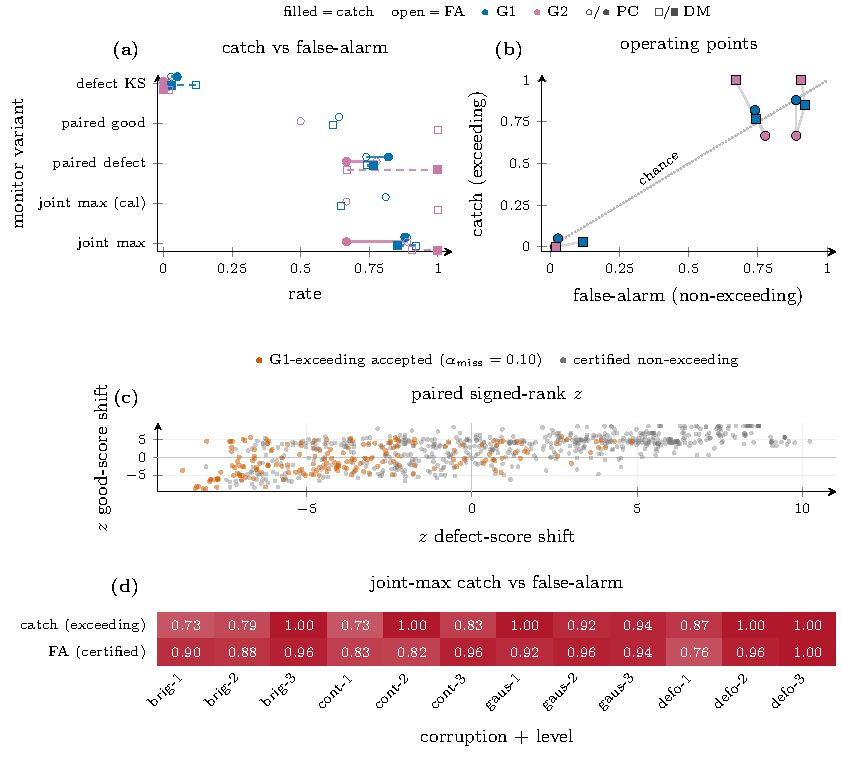
\includegraphics[width=0.97\linewidth,height=0.55\textheight,keepaspectratio]{figures/fig-jointmon.pdf}
\caption{The drift-monitor design space, tested (post-freeze exploratory, seed 0; frozen joint
record). \textbf{a:} catch rate (filled) vs.\ false-alarm rate (open) per monitor variant and
detector$\times$guarantee arm --- the frozen defect-marginal KS catches $5.0\%$/$2.9\%$; the
pairing-respecting variants catch more but at matching false-alarm. \textbf{b:} the same arms as
operating points against the chance diagonal: no variant separates. \textbf{c:} per-cell paired
signed-rank $z$ of good- and defect-score shifts; G1-exceeding accepted cells (vermillion) sit
inside the same cloud as certified cells --- there is no location-only signature to detect.
\textbf{d:} catch vs.\ false-alarm rate of the joint max-statistic by corruption and severity
level: the two rows track each other at every cell, the indiscriminate regime in one view. From
the frozen joint-monitor record (792 cells; reproduction gates passed: defect-marginal catches
$5/100$ and $1/34$ reproduced exactly).}\label{fig:jointmon}
% source: drift_joint_monitor_2026-08-01/results.json
% figure: manuscripts/figures-src/R/jointmon.R + tikz/fig-jointmon.tex
\end{figure}

Calibrated gates also do not transfer across detectors. The gate is calibrated per detector, and
a threshold-transfer experiment (post-freeze exploratory, seed-level) shows that requirement is
not cosmetic. Calibrating on
PatchCore's calibration-half scores and applying the thresholds to Dinomaly's evaluation-half
scores --- the identical images, labels, and stratified partition, so the only change is the
scoring function --- violates the escaped-defect guarantee in $160/165$ cells across the three
benchmarks (up to $+87$ points above the $\alpha_{\text{miss}}$ tolerance); the reverse
direction violates the false-reject guarantee in $80/165$ cells. The same-detector diagonal
reproduces the frozen certification records exactly ($30/30$ cells, with a perturbation
negative control), so the failure is the transfer, not the harness. This is a model-shift axis,
complementary to --- and easier than --- the temporal threshold-transfer across production
periods named above as future work: even swapping the scoring function on fixed data breaks the
certificate. A deployed gate must therefore be recalibrated against the detector it guards, and
any detector upgrade re-opens calibration; on VisA the comparison is additionally not
architecture-controlled (Dinomaly is a single multi-class model across all twelve categories,
PatchCore per-category), so the transfer figures there are descriptive
(Figure~\ref{fig:xdet}).

\begin{figure}[tbp]\centering
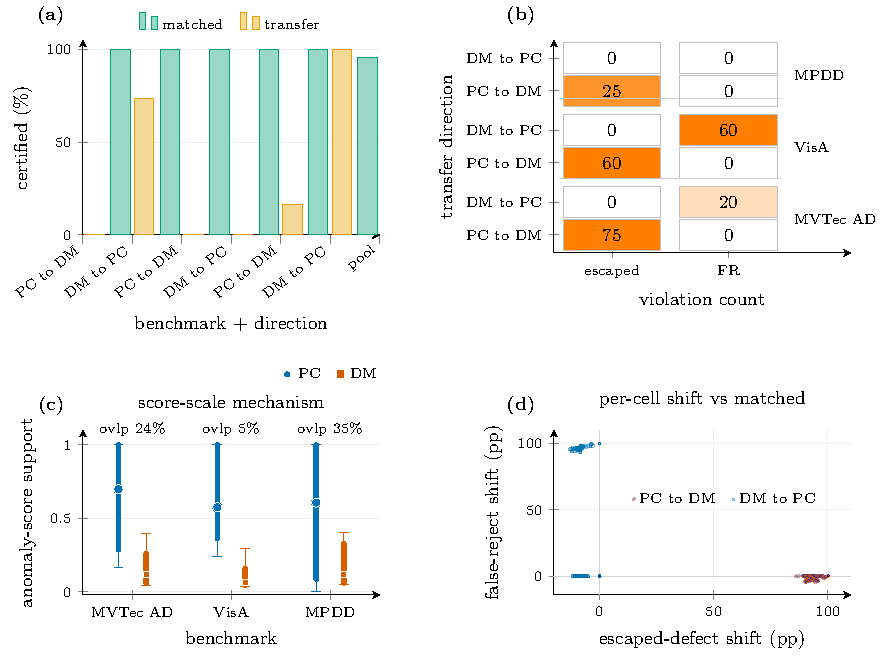
\includegraphics[width=\linewidth,height=0.55\textheight,keepaspectratio]{figures/fig-xdet.pdf}
\caption{Calibrated gates do not transfer across detectors (post-freeze exploratory,
seed-level; frozen transfer record). \textbf{a:} certification rate, transfer vs.\
partition-matched same-detector diagonal, per benchmark and direction --- the diagonal
certifies nearly everywhere; the transfer arm collapses. \textbf{b:} guarantee-violation
counts per benchmark and direction: $160/165$ escaped-defect violations
(PatchCore$\to$Dinomaly, abbreviated ``PC to DM'' in the figure), $80/165$ false-reject
violations (reverse, ``DM to PC''). \textbf{c:} the
mechanism --- per-detector score-scale ranges barely overlap (support overlap
$0.241$/$0.053$/$0.353$ on MVTec AD/VisA/MPDD), so a threshold calibrated on one
detector sits far outside the other's score support. \textbf{d:} per-cell realized-rate
shift vs.\ the matched diagonal; the two clusters show total inversion in opposite
directions. From the frozen transfer record (330 cells; same-detector diagonal
reproduces the frozen certification records exactly, 30/30).}\label{fig:xdet}
% source: cross_detector_transfer_2026-08-01/results.json via R/xdet.R -> tikz/fig-xdet.tex (pure R/CSV/TikZ pipeline)
\end{figure}

Small good-calibration pools are intended behavior, not a shortfall: G2's certifiable count is a
direct property of each benchmark's good-pool size, not a conservatism baked into the gate.
MVTec AD ($4/15$), VisA ($12/12$, identical code path), and MPDD ($0/6$ under the primary
protocol, rescued to $4/6$ under the flag-gated train-holdout arm) form three points consistent
with pool-size-driven refusal (Sections~\ref{sec:floors}, \ref{sec:mpddholdout}). MPDD's rescue is
PatchCore-only because no MPDD Dinomaly train-score dump exists; the later MVTec/VisA Dinomaly
dumps are checkpoint-dependent exploratory sensitivities and do not alter that evidence boundary.

The near-universal G1 certification reported above ($15/15$ MVTec AD, $12/12$ VisA, $5/6$ MPDD)
holds at $\alpha_{\text{miss}}=0.10$ --- a $10\%$ chance of auto-passing a defective part, well
outside what a safety-critical line would accept --- and is an artifact of that tolerance being
easy to clear against the $\alpha_{\min}=1/(n_{\text{cal}}^{\text{def}}+1)$ floor at these
benchmarks' defect-calibration pools ($n_{\text{cal}}^{\text{def}}\in[15,70]$ on MVTec AD,
Table~\ref{tab:floors}; $=50$ on VisA; $\in[7,36]$ on MPDD). At a deployable tolerance of
$\alpha_{\text{miss}}=0.01$ the floor requires $n_{\text{cal}}^{\text{def}}\ge 99$, which no
category on any of the three benchmarks reaches, so G1 refuses in all $33/33$ (benchmark,
category) cells; at $\alpha_{\text{miss}}=0.001$ ($n_{\text{cal}}^{\text{def}}\ge 999$) the same
is true. The full operating-point frontier is now computed, not just this boundary arithmetic
(Figure~\ref{fig:alphafrontier}; post-freeze exploratory sweep of
$\alpha_{\text{miss}}\in\{0.20,\dots,0.01\}\times\alpha_{\text{fr}}\in\{0.10,0.05,0.02\}$ on the
frozen code path, verified to reproduce every frozen artifact exactly at the paper's operating
point): VisA certifies both axes in $12/12$ categories down to $\alpha_{\text{miss}}=0.02$ at
modest deferral cost (Dinomaly $6.5\%\!\to\!12.9\%$) before the floors bind and certification
collapses to $0/12$ at $0.01$; MVTec AD's both-axis fraction is pinned at $4/15$ by the
good-pool floors across $\alpha_{\text{miss}}\ge 0.05$ regardless of tolerance; MPDD certifies
nothing at any grid point on the primary protocol. The sweep confirms the refusal collapse is
exactly where the floor arithmetic predicts, and prices every reachable tighter point. On
academic benchmarks of this size, the meaningful demonstration is the refusal discipline itself
--- that the gate honestly refuses rather than assert an escape guarantee the data cannot support
--- not a certified industrially-tight escape rate. Certifying escaped-defect at the
$1\%$--$0.1\%$ tolerances a safety-critical line would require needs the larger
labeled-defective pools (hundreds to thousands per category) that accrue from rework and scrap
logging over months of production (Section~\ref{sec:gate}), not the few dozen defective images an
academic test split provides.

% Flush the two preceding [t] floats (jointmon, xdet) within the Results section
% so they land within one page of their citations instead of deferring past the
% Conclusion into the appendix float pages.
\FloatBarrier

\section{Conclusion}
\label{sec:conclusion}

We described a pre-deployment three-way triage gate that turns anomaly-detector scores into an
auditable benchmark operating decision with finite-sample escaped-defect and false-reject guarantees, and a
refusal mechanism that makes ``not enough data to certify'' a visible outcome. The framework is not yet a
factory-validated deployment: the reported operating point is $\alpha_{\text{miss}}=0.10$, all $33$
benchmark categories refuse at $0.01$, and production-line drift remains untested. Its engineering value is
the explicit calibration-data requirement, priced deferral, and refusal discipline that must be resolved
before a line can claim a tighter certificate. On MVTec AD,
VisA, and MPDD, across two backbones and five seeds each, the calibration machinery matches its
preregistered arithmetic exactly, with no kill-gate tripped in any of the $30$ (backbone, seed)
aggregates. The three benchmarks exercise complementary failure modes and together give three
points consistent with pool-size-driven refusal ($0/6 \to 4/15 \to 12/12$): MVTec AD
stresses the refusal side (G2 certifiable in only $4/15$ categories under the primary protocol,
lifted to $12$--$13/15$ by the frozen train-holdout remedy --- PatchCore-only because the
eligible independent holdout is unavailable for Dinomaly --- with KS-failing categories honestly refused);
VisA --- lower-ceiling, larger good pools --- certifies both axes in all $12$ categories,
cuts median deferral to $4$--$19\%$, and gives the excess-AURC audit the headroom MVTec's
saturated backbones deny it; and MPDD (real painted-metal parts, post-freeze exploratory) is the
stingy extreme, refusing G2 in all $6$ categories under the primary protocol and rescued to $4/6$
by the flag-gated train-holdout arm (one category KS-audited out). The confirmatory pooled audit
(C2) returns a constructive verdict on
MVTec AD --- field-standard threshold practice earns real deferral skill over honest random deferral
in all five backbone seeds (Section~\ref{sec:c2}).

\section*{Data availability}
MVTec AD~\citep{bergmann2019mvtec}, VisA~\citep{zou2022spot}, and
MPDD~\citep{jezek2021mpdd} are publicly available benchmarks. Code, frozen analysis digests, and
reproducibility manuals (including the preregistration freeze log) for this study are archived at
Zenodo (concept DOI
\href{https://doi.org/10.5281/zenodo.21392290}{\texttt{10.5281/zenodo.21392290}};
version~0.4.1, record DOI \texttt{10.5281/zenodo.21854312}) and maintained at
\url{https://github.com/PeterPonyu/inspect-gate}.

\section*{Declaration of competing interest}
The author declares no known competing financial interests or personal relationships
that could have appeared to influence the work reported in this paper.

\section*{Declaration of generative AI in scientific writing}
Generative AI tools were used during manuscript preparation. The author reviewed and edited
the resulting content and takes full responsibility for the published article.

\section*{Funding}
The author received no funding for this work.

\section*{CRediT authorship contribution statement}
Zeyu Fu: Conceptualization, Methodology, Software, Validation, Formal analysis, Investigation, Data
curation, Writing -- original draft, Writing -- review \& editing, Visualization.

\appendix
% Restart figure/table numbering for the appendix so supplementary floats are
% labelled A.1, A.2, ... (continuing the main-text counter would mislabel them
% A.17, A.18 / A.10, A.11, which does not match first-appearance order within
% the appendix).
\setcounter{figure}{0}
\setcounter{table}{0}
\section{Supplementary tables and figures}
\label{app:supp}

% Tall Mondrian heatmaps first so each can use a shared horizontal scale without
% competing with the bridge prose for vertical space. Both use width=0.67\linewidth
% (≈ part 2's former effective width under height=0.82\textheight+keepaspectratio);
% the old height=0.48\textheight cap on part 1 made keepaspectratio shrink it far
% below part 2 and left large side margins.
\begin{figure}[H]
\centering
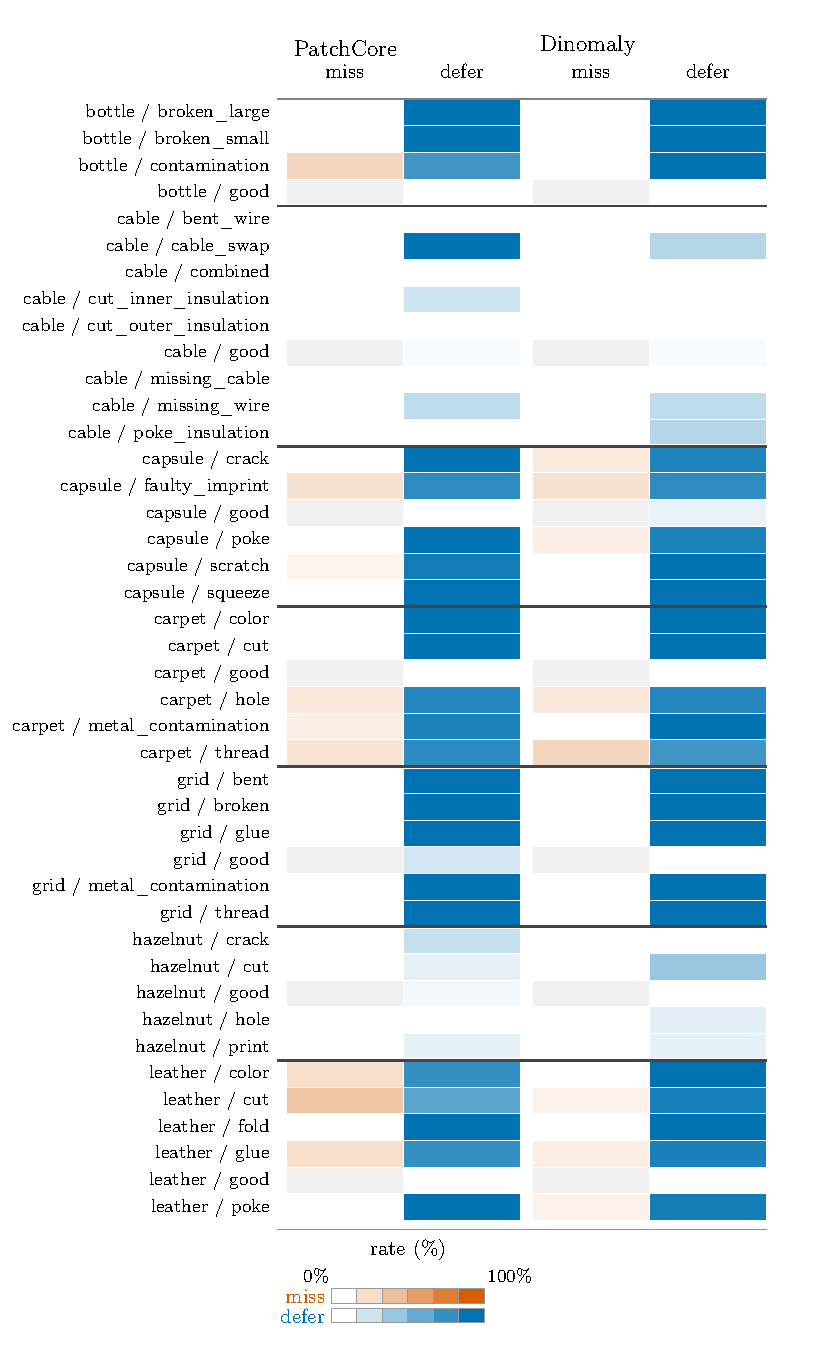
\includegraphics[width=0.67\linewidth]{figures/fig-mondrian-1.pdf}
\caption{Defect-type Mondrian map, part 1 (bottle--leather). Per (category,
defect-type): realized escaped-defect (miss) rate among defective eval images
(left column, vermillion) and deferral rate over all eval images (right column,
blue), for both backbones at the operating point (seed 0, repeat 0; post-freeze
exploratory). Cell shade encodes the rate; per-cell counts ($n_{\text{def}}$, $n$)
live in the frozen archive. White miss cells mean zero observed misses or an
undefined rate when $n_{\text{def}}=0$. Residual errors concentrate in specific
subtle-appearance defect types (e.g.\ pill::color, leather::cut) rather than
uniformly. Horizontal separators mark category boundaries in both backbone panels.}
\label{fig:mondrian1}
\end{figure}

\begin{figure}[H]
\centering

\includegraphics[width=0.67\linewidth]{figures/fig-mondrian-2.pdf}
\caption{Defect-type Mondrian map, part 2 (metal\_nut--zipper). Encoding as in
Figure~\ref{fig:mondrian1}.}
\label{fig:mondrian2}
\end{figure}

The three appendix tables below were moved out of the main text to keep the Results
section readable; every main-text reference to them resolves here.
Figures~\ref{fig:mondrian1}--\ref{fig:mondrian2} give the defect-type (Mondrian)
coverage map for MVTec AD (VisA's public ground truth carries a single ``bad''
stratum per category and MPDD is reported per category).

\begin{table}[htbp]
  \centering
  \small
  \caption{Per-category certifiability at $\alpha_{\text{miss}}=0.10$, $\alpha_{\text{fr}}=0.05$
  (backbone-invariant; pure functions of the shared MVTec test split). G1 certifies in $15/15$,
  G2 in $4/15$. Source: the frozen preregistration (\S3), reproduced with $0/15$ mismatch by the
  analysis pipeline.}
  % source: PREREG-DRAFT-2026-07-10.md §3; recomputed by run_analysis.py
  \label{tab:floors}
  \begin{tabular}{lccccc}
    \toprule
    Category & $n_{\text{cal}}^{\text{def}}$ & $\alpha_{\min}$(G1) & G1@0.10 & $n_{\text{cal}}^{\text{good}}$ & G2@0.05 \\
    \midrule
    bottle     & 32 & 0.0303 & OK & 10 & REFUSE \\
    cable      & 46 & 0.0213 & OK & 29 & OK \\
    capsule    & 54 & 0.0182 & OK & 12 & REFUSE \\
    carpet     & 44 & 0.0222 & OK & 14 & REFUSE \\
    grid       & 28 & 0.0345 & OK & 10 & REFUSE \\
    hazelnut   & 35 & 0.0278 & OK & 20 & OK \\
    leather    & 46 & 0.0213 & OK & 16 & REFUSE \\
    metal\_nut & 46 & 0.0213 & OK & 11 & REFUSE \\
    pill       & 70 & 0.0141 & OK & 13 & REFUSE \\
    screw      & 60 & 0.0164 & OK & 20 & OK \\
    tile       & 42 & 0.0233 & OK & 16 & REFUSE \\
    toothbrush & 15 & 0.0625 & OK & 6  & REFUSE \\
    transistor & 20 & 0.0476 & OK & 30 & OK \\
    wood       & 30 & 0.0323 & OK & 10 & REFUSE \\
    zipper     & 60 & 0.0164 & OK & 16 & REFUSE \\
    \midrule
    \multicolumn{3}{l}{\textbf{Certifiable}} & 15/15 & & 4/15 \\
    \bottomrule
  \end{tabular}
\end{table}

\begin{table}[htbp]
  \centering
  \small
  \caption{Seed-$0$ median per-category deferral by benchmark and backbone
  (Section~\ref{sec:v1res}), with the mean where computed and the extreme categories. G2 refusal
  (Section~\ref{sec:floors}) empties the auto-reject band and elevates deferral on MVTec AD and
  MPDD; VisA's universal G2 certification keeps deferral low.}
  \label{tab:deferral}
  \resizebox{\linewidth}{!}{%
  \begin{tabular}{llcccc}
    \toprule
    Benchmark & Backbone & Median & Mean & Max category & Min category \\
    \midrule
    MVTec AD & PatchCore & $70.0\%$ & $55.1\%$ & pill $78.0\%$ & transistor $2.0\%$ \\
    MVTec AD & Dinomaly  & $69.5\%$ & $54.2\%$ & capsule $77.3\%$ & screw $3.1\%$ \\
    VisA     & PatchCore & $18.7\%$ & ---      & macaroni2 $72.5\%$ & chewinggum $2.0\%$ \\
    VisA     & Dinomaly  & $4.2\%$  & ---      & capsules $21.9\%$ & candle $2.5\%$ \\
    MPDD     & PatchCore & $74.1\%$ & ---      & connector $100\%$ & bracket brown $61.8\%$ \\
    MPDD     & Dinomaly  & $70.9\%$ & ---      & connector $100\%$ & bracket white $53.3\%$ \\
    \bottomrule
  \end{tabular}%
  }
\end{table}

\begin{table}[h!]
  \centering
  \small
  \caption{Per-backbone companion to Table~\ref{tab:crcbaseline}: our dual gate vs.\ the CRC
  single-threshold baseline, pooled over five seeds and all categories per backbone (point rates;
  per-seed min--max bands are included in the published analysis archive). CRC has no
  deferral mechanism and no G2 certificate by construction.}
  \label{tab:crcbackbone}
  % source: baseline_comparison_2026-07-15/results.json per_backbone blocks
  \begin{tabular}{@{}lllcccc@{}}
    \toprule
    Benchmark & Backbone & Method & Escaped & False-reject & Deferral \\
    \midrule
    MPDD & PatchCore & Our dual gate & $7.1\%$ & $0.0\%$ & $75.1\%$ \\
    MPDD & PatchCore & CRC & $7.1\%$ & $41.9\%$ & $0.0\%$ \\
    MPDD & Dinomaly  & Our dual gate & $6.1\%$ & $0.0\%$ & $71.1\%$ \\
    MPDD & Dinomaly  & CRC & $6.1\%$ & $31.8\%$ & $0.0\%$ \\
    \addlinespace
    VisA & PatchCore & Our dual gate & $8.8\%$ & $3.7\%$ & $26.3\%$ \\
    VisA & PatchCore & CRC & $9.7\%$ & $28.8\%$ & $0.0\%$ \\
    VisA & Dinomaly  & Our dual gate & $6.5\%$ & $2.2\%$ & $6.5\%$ \\
    VisA & Dinomaly  & CRC & $9.3\%$ & $3.7\%$ & $0.0\%$ \\
    \addlinespace
    MVTec AD & PatchCore & Our dual gate & $7.7\%$ & $0.7\%$ & $54.8\%$ \\
    MVTec AD & PatchCore & CRC & $8.4\%$ & $5.2\%$ & $0.0\%$ \\
    MVTec AD & Dinomaly  & Our dual gate & $6.9\%$ & $0.3\%$ & $53.9\%$ \\
    MVTec AD & Dinomaly  & CRC & $8.7\%$ & $0.9\%$ & $0.0\%$ \\
    \bottomrule
  \end{tabular}
\end{table}

\begin{table}[htbp]
  \centering
  \small
  \caption{V1 tier-2 grading, per category (expanded from the aggregate axis totals in the text;
  every cell out of $10=2$ backbones$\,\times\,5$ seeds). Escaped-defect is pass/fail/unpowered
  against the per-repeat $0.13$ Clopper--Pearson bound (amendment A2); false-reject is
  pass/fail/unpowered/refused, where ``refused'' means the category is not G2-certified
  (amendment A3) and ``unpowered'' means it is G2-certified but fails the per-repeat power floor
  (amendment A1). MVTec AD is $0$-gradeable on false-reject by construction (no G2-certified
  category clears the power floor); VisA (post-freeze, exploratory) is partially gradeable.}
  \label{tab:tier2}
  \resizebox{\linewidth}{!}{%
  \begin{tabular}{@{}lcc@{}}
    \toprule
    Category & Escaped-defect (pass/fail/unpwr.) & False-reject (pass/fail/unpwr./refused) \\
    \midrule
    \multicolumn{3}{@{}l}{\emph{MVTec AD (confirmatory tier-1 family; amendments A1/A2/A3)}} \\
    bottle     & $0/10/0$ & $0/0/0/10$ \\
    cable      & $5/5/0$  & $0/0/10/0$ \\
    capsule    & $0/10/0$ & $0/0/0/10$ \\
    carpet     & $0/10/0$ & $0/0/0/10$ \\
    grid       & $0/10/0$ & $0/0/0/10$ \\
    hazelnut   & $10/0/0$ & $0/0/10/0$ \\
    leather    & $0/10/0$ & $0/0/0/10$ \\
    metal\_nut & $0/10/0$ & $0/0/0/10$ \\
    pill       & $0/10/0$ & $0/0/0/10$ \\
    screw      & $0/10/0$ & $0/0/10/0$ \\
    tile       & $0/10/0$ & $0/0/0/10$ \\
    toothbrush & $0/0/10$ & $0/0/0/10$ \\
    transistor & $0/0/10$ & $0/0/10/0$ \\
    wood       & $0/10/0$ & $0/0/0/10$ \\
    zipper     & $0/10/0$ & $0/0/0/10$ \\
    \midrule
    \multicolumn{3}{@{}l}{\emph{VisA (post-freeze, exploratory)}} \\
    candle      & $0/10/0$ & $0/10/0/0$ \\
    capsules    & $0/10/0$ & $0/0/10/0$ \\
    cashew      & $0/10/0$ & $0/0/10/0$ \\
    chewinggum  & $10/0/0$ & $0/0/10/0$ \\
    fryum       & $0/10/0$ & $0/0/10/0$ \\
    macaroni1   & $0/10/0$ & $0/10/0/0$ \\
    macaroni2   & $0/10/0$ & $0/10/0/0$ \\
    pcb1        & $0/10/0$ & $0/10/0/0$ \\
    pcb2        & $0/10/0$ & $0/10/0/0$ \\
    pcb3        & $0/10/0$ & $0/10/0/0$ \\
    pcb4        & $5/5/0$  & $4/6/0/0$ \\
    pipe\_fryum & $2/8/0$  & $0/0/10/0$ \\
    \midrule
    \multicolumn{3}{@{}l}{\textbf{Totals}} \\
    MVTec AD (150 cells) & $15/115/20$ & $0/0/40/110$ \\
    VisA (120 cells)     & $17/103/0$  & $4/66/50/0$ \\
    \bottomrule
  \end{tabular}%
  }
  % source: c2_tier2_2026-07-13/tier2_mvtec.json, tier2_visa.json (per_cell breakdown,
  % aggregated per category over 2 backbones x 5 seeds; totals cross-checked against the
  % benchmark-level escaped_axis/false_reject_axis counts already cited in the text)
\end{table}

\FloatBarrier
\bibliographystyle{elsarticle-num}
\bibliography{refs}

\end{document}
